\documentclass{article}
\usepackage{blindtext}
\usepackage{titlesec}
\usepackage{graphicx}
\usepackage{amsmath}
\usepackage{amsfonts}
\usepackage[margin=1in]{geometry}
\usepackage{adjustbox}
\usepackage[
backend=biber,
style=numeric,
]{biblatex} 
\usepackage{booktabs}
\usepackage{hyperref}
\usepackage{enumitem}
\usepackage[section]{placeins}

\addbibresource{references.bib}
\graphicspath{ {./images/} }

\title{ChordSeqAI: Generating Chord Sequences Using Deep Learning}
\author{Petr Ivan}
\date{December 2023}

\begin{document}

\newpage

\maketitle

\begin{abstract}
This report presents a novel AI-driven tool for aiding musical composition through the generation of chord progressions. Data acquisition and analysis are discussed, uncovering intriguing patterns in chord progressions across diverse musical genres and periods. We developed a range of deep learning models, from basic recurrent networks to sophisticated Transformer architectures, including conditional and style-based Transformers for improved controllability. Human evaluation indicates that, within the context of our specific data processing methods, the chord sequences generated by the more advanced models are practically indistinguishable from real sequences. The models are then integrated into a user-friendly open-source web application, making advanced music composition tools accessible to a broader audience.
\end{abstract}

\tableofcontents

\newpage

\section{Introduction}

\subsection{Music Theory Background}

Music composition is intricately tied to the foundations of music theory, among which chord progressions play a crucial role. One must first delve into the musical context to comprehend the intricacies of chord sequence generation. Contemporary music is comprised of a few vital elements, including the overall structure, rhythm, melody, harmony, timbre, and dynamics. Harmony can be conceptualized as multiple melodies creating a polyphonic texture. However, recent trends in musical composition have seen a shift in this perspective, with harmony often being treated as an independent entity and the melodies forming them assuming a comparatively subordinate role than historically. 

The fundamental building block of harmony became a chord - a group of notes sounded together. A basic form, a cornerstone of Western music, is the triad, made from the root, third and fifth. The most common are major, minor, diminished, and augmented triads, differing in the interval used for them. Beyond these, various other chords exist, formed through diverse methods such as upper chord extensions (notably seventh, eleventh, and thirteenth chords, along with their variants), suspensions (resulting in sus2 and sus4 chords), or slash chords (that have an added bass tone).

An interesting aspect of chords is their notation. Usually, a chord symbol contains the root note, the quality of the chord (indicating if it is major, minor, diminished, etc.), any altered or added notes, and the bass if it differs from the root. Symbolic representation of chords is not standardized; instead, various notations are employed depending on the context. For instance, a major seventh chord can be represented by maj7, M7, $\Delta$7, or even just ma7 or $\Delta$. This work attempts to use an unambiguous chord notation; pitches are described by the Scientific pitch notation (also known as the American standard pitch notation).

Chord progressions, then, are a series of such chords played in a sequence. The progressions, also referred to as sequences in certain contexts, are not random; rather, they follow specific patterns and rules that have evolved over centuries of musical tradition. The beauty of chord progressions lies in their versatility and expressiveness, where each progression carries its unique mood and character. One of the key concepts in understanding chord progressions is the idea of tonality, which refers to the way chords are centered around a tonic, or home key. This concept gives rise to the notion of diatonic chords, that are built from the notes of a single key. These chords are typically labeled with Roman numerals, which denote their position in the tonic (commonly, uppercase numerals represent major chords and lowercase minor). In this fashion, we can describe some common chord progressions, including ii-V-I, I-IV-V, or I-V-iv-IV  (see section \ref{EDA} for more examples).

Another important aspect of chords is their inversions and voicings when describing the progressions. Inversions refer to variants of the chord with a different bass but the same notes (commonly constructed by moving the lowest notes an octave up with triad chords), while voicings refer to the melodic changes of each voice as in the polyphonic view (usually by using different chord inversions to minimalize the distance between the notes, or moving the voices in a certain direction).

Less experienced musicians often use melody or harmony-first approaches to music composition, while more experienced use a more hybrid approach, often focusing on multiple aspects of the music at the same time, as the separate creation of the individual aspects has its limitations (e.g. melody-first approach often produces too simple harmonies, while harmony-first often lacks voice leading and the melodies can be limited). The composition of harmony is not a primitive task, as the standard methods of finding chords fitting into the context produce a large space of possibilities (such as by the circle of fifths, diatonic chords, or secondary dominants), which is difficult to navigate. Furthermore, when we get into more complex chord progressions with upper chord extensions and other alterations, the space, as well as the rules, become broader, and experience remains the only means of a sense of direction.

Instead of deriving the general harmony composition rules, we can develop deep learning models that will learn chord progressions to navigate us. Through this project, we attempted to help those beginning their journey into music composition by providing a powerful AI-driven assistant for the creation of chord sequences, helping them explore the space of possibilities and making the harmony-first approach more accessible.

\subsection{Deep Learning in Music Generation}

We can classify the common research areas in a few ways. Based on the representation of the data used, there are symbolic (e.g. learning from MIDI files) and sub-symbolic (e.g. given a spectrogram of an audio file) approaches. Different objectives exist, including generating melody \cite{DBLP:journals/corr/abs-2109-00663}, harmony \cite{9053992, dalmazzo2023chordinator, 8554901}, polyphony \cite{DBLP:journals/corr/abs-1710-11418}, \cite{DBLP:journals/corr/abs-1804-09399}, accompaniment \cite{10.1145/3394171.3413721, 10.1145/1357054.1357169, Jiang_Jin_Duan_Zhang_2020}, or synthesizing the raw audio \cite{mubert2022, forsgren2022riffusion, agostinelli2023musiclm}).

Simple Markov chains were quite commonly used until the advent of deep learning. Then feed-forward neural networks came, followed by (variational) autoencoders, recurrent neural networks, convolutional neural networks, generative adversarial networks, and reinforcement learning approaches \cite{DBLP:journals/corr/abs-1709-01620}. Recent works also explore the use of the Transformer architecture \cite{https://doi.org/10.1049/cit2.12065, dhariwal2020jukebox, 9768298, Muhamed_Li_Shi_Yaddanapudi_Chi_Jackson_Suresh_Lipton_Smola_2021}).

Our work focuses on raw harmony generation (without a reference melody), which falls under symbolic music generation. The use of machine learning on this task is not new, for example, \cite{huang16chordripple} demonstrated a way to recommend chords with a WordToVec approach on a corpus of chord progressions. \cite{dalmazzo:hal-04289026} presented a way to model chord progressions using the Transformer, while \cite{8554901} employed a reinforcement learning technique. Other, non-deep learning strategies, exist, such as those using evolutionary algorithms \cite{10.1007/978-3-319-13560-1_69}, artificial immune systems \cite{NAVARROCACERES2019100543}, or rule-based methods \cite{doi:10.1080/09298215.2016.1173708}. Many of these tools are not easily accessible to the public, are limited in terms of the number of different chords, or lack controllability. In this graduate project, we attempted to overcome many of the limitations of these techniques.

For an in-depth overview of deep learning in music generation, you can check out \cite{DBLP:journals/corr/abs-1709-01620}.

\section{Data}

\subsection{Data Acquisition}

Since the performance of any model strongly correlates with the quality and diversity of the data it was trained on, acquiring a high-quality dataset is essential. There are not many freely available large enough datasets of chord sequences, though a few options exist, such as the McGill Billboard dataset, which contains 700 entries \cite{burgoyne2011expert}. To get interesting results, we need our dataset to be significantly larger.

Instead of merging multiple datasets, we decided to obtain our own from web pages containing songs annotated with chords. In particular, Ultimate Guitar was chosen for its enormous collection of over a million songs \cite{ultimateguitar}. In addition to the chords, this website also contains ways of acquiring additional data about the songs, such as their genre, decade, or style. Although we cannot directly view this info once a tab is open, we can filter through the songs and get it this way. The filters applied are specified in the URL allowing us to easily navigate through them. The notes of each chord are also sent over the network (as a JSON file with MIDI note numbers) upon opening piano chords in the tab, which will turn out to be useful during tokenization, as described in section \ref{Data Tokenization}.

A scraper was written in Python with the Playwright library \cite{playwright}. Given a limited computing capacity, only up to the first 300 entries by rating were scraped for each genre across every decade, forming a decent dataset of 22,367 samples after cleanup. Some combinations of genres and decades contained less than 300 entries, while others were vastly larger and could be scraped further to extend the dataset. This approach gave us data that encompasses even the less popular genres without requiring much computing power. Scraping was done at a slower pace, it took a few dozen hours, and rate limitations were not hit. The scraper, as well as all other code, data, and additional resources, are available on GitHub (see section \ref{Resources}),

Ethical considerations come into play when using the artworks of others for training AI models. Generally, melodies, as well as the lyrics of a song, are protected as they are considered unique works of the composer or lyricist, while chord progressions are not typically subject to copyright. This is because of the limited space of possible progressions fitting into the mood and genre of the song, so many songs use the same ones \cite{EasySong2023Copyright}. Nevertheless, we want to make sure that the models produce novel sequences and not just blindly replicate the training data.

\subsection{Exploratory Data Analysis} \label{EDA}

Given the raw data, duplicates and incomplete samples were removed. When a song is associated with more than a single genre, it shows up in multiple entries that can be merged. These genres in a merged entry were then separated by a vertical bar because spaces, commas, and other common separation characters were already present in the genre names. To ensure that we have usable data, we constructed a complete chord map from all of the individual notes per chord symbol obtained during scraping. Since sometimes not all chords of a song were present in the data, the map was then transposed into all possible keys using music21 library \cite{music21}. Entries that contained any chords not present in the complete chord map were removed. Such entries had a generally lower number of ratings as well as the number of stars, which Ultimate Guitar users use to rate the accuracy of the chords used. Note that it was verified that there are no ambiguous chord symbols (that would be represented with different notes). This processing reduced the total number of entries from 32,792 to 22,367 (most being duplicates). Low-quality data, indicated by either a low number of stars or ratings, could also be removed, however, since we did not have additional measures to ensure that they were not simply unpopular but still valuable data, they were kept. Consecutive chords were also merged, as we only care about harmonic changes.

\begin{figure}[!htbp]
    \centering
    \begin{minipage}{.49\textwidth}
        \centering
        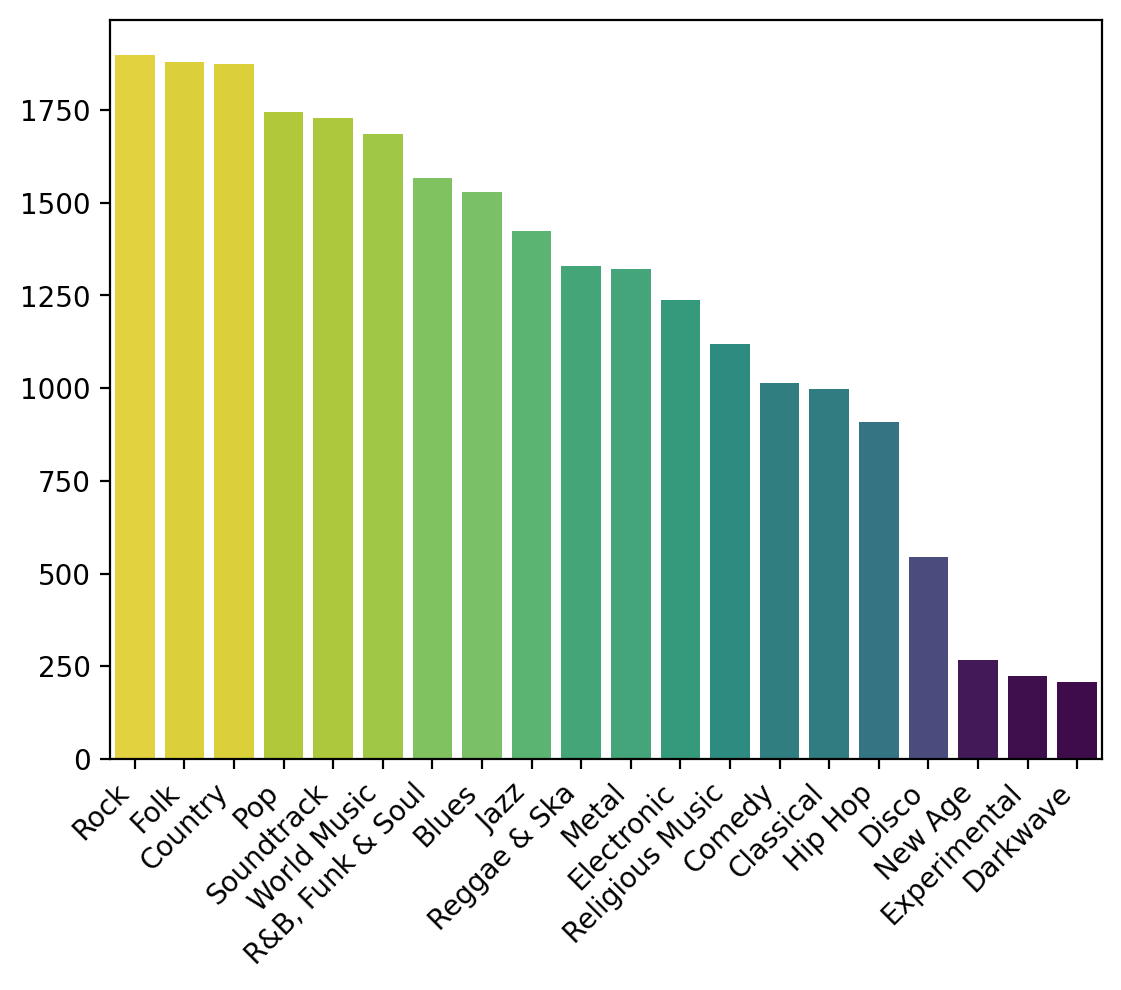
\includegraphics[width=\linewidth]{images/genre-distribution.png}
    \end{minipage}\hfill
    \begin{minipage}{.49\textwidth}
        \centering
        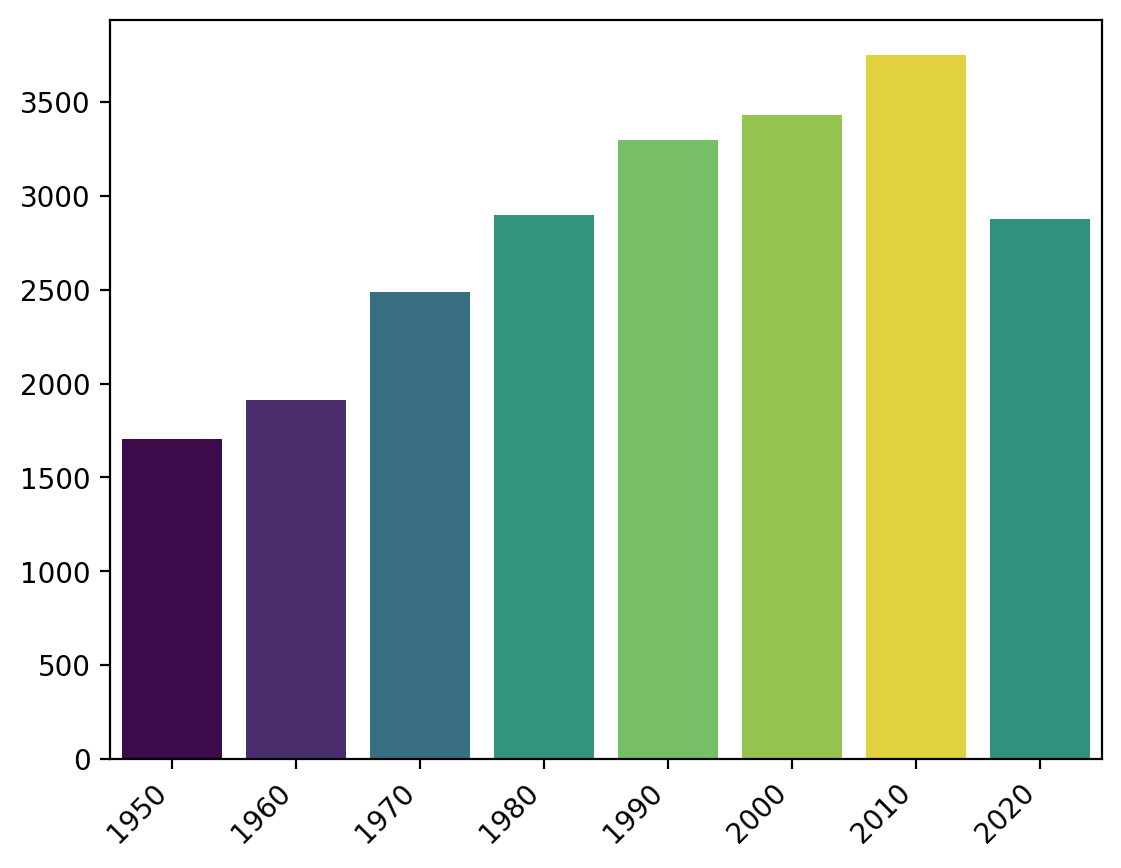
\includegraphics[width=\linewidth]{images/decade-distribution.png}
        \vspace{0.475cm}
    \end{minipage}
    \caption{The distribution of genres and decades in the dataset.}
    \label{fig:genre-decade-distribution}
\end{figure}

We can plot the distribution of individual genres and decades in the dataset, as visualized in Figure \ref{fig:genre-decade-distribution}. We seem to get a balanced dataset, with only a few genres being underrepresented. There are more new songs than old ones, except for the current decade (as it is still ongoing).

Before delving into the chord progressions, we visualized the usage of individual chords - their root note (without merging enharmonically equivalent notes) and the form of the chord, called the extension for simplicity here (see Figure \ref{fig:roots-extensions-across-genres}). Slash chords were normalized to have relative meaning (represented by Roman numerals), as the function of the slash part strongly depends on the root. To better see the more subtle details, logarithmically normalized plots were created. It shows us a strong dark stripe among the different extensions and roots used in Jazz, while Country and Darkwave show the opposite. Some interesting observations can be made from the individual forms used, such as that Metal is the only genre that extensively uses power chords (denoted by a 5).

\begin{figure}[!htbp]
    \centering
    \begin{minipage}{\textwidth}
        \centering
        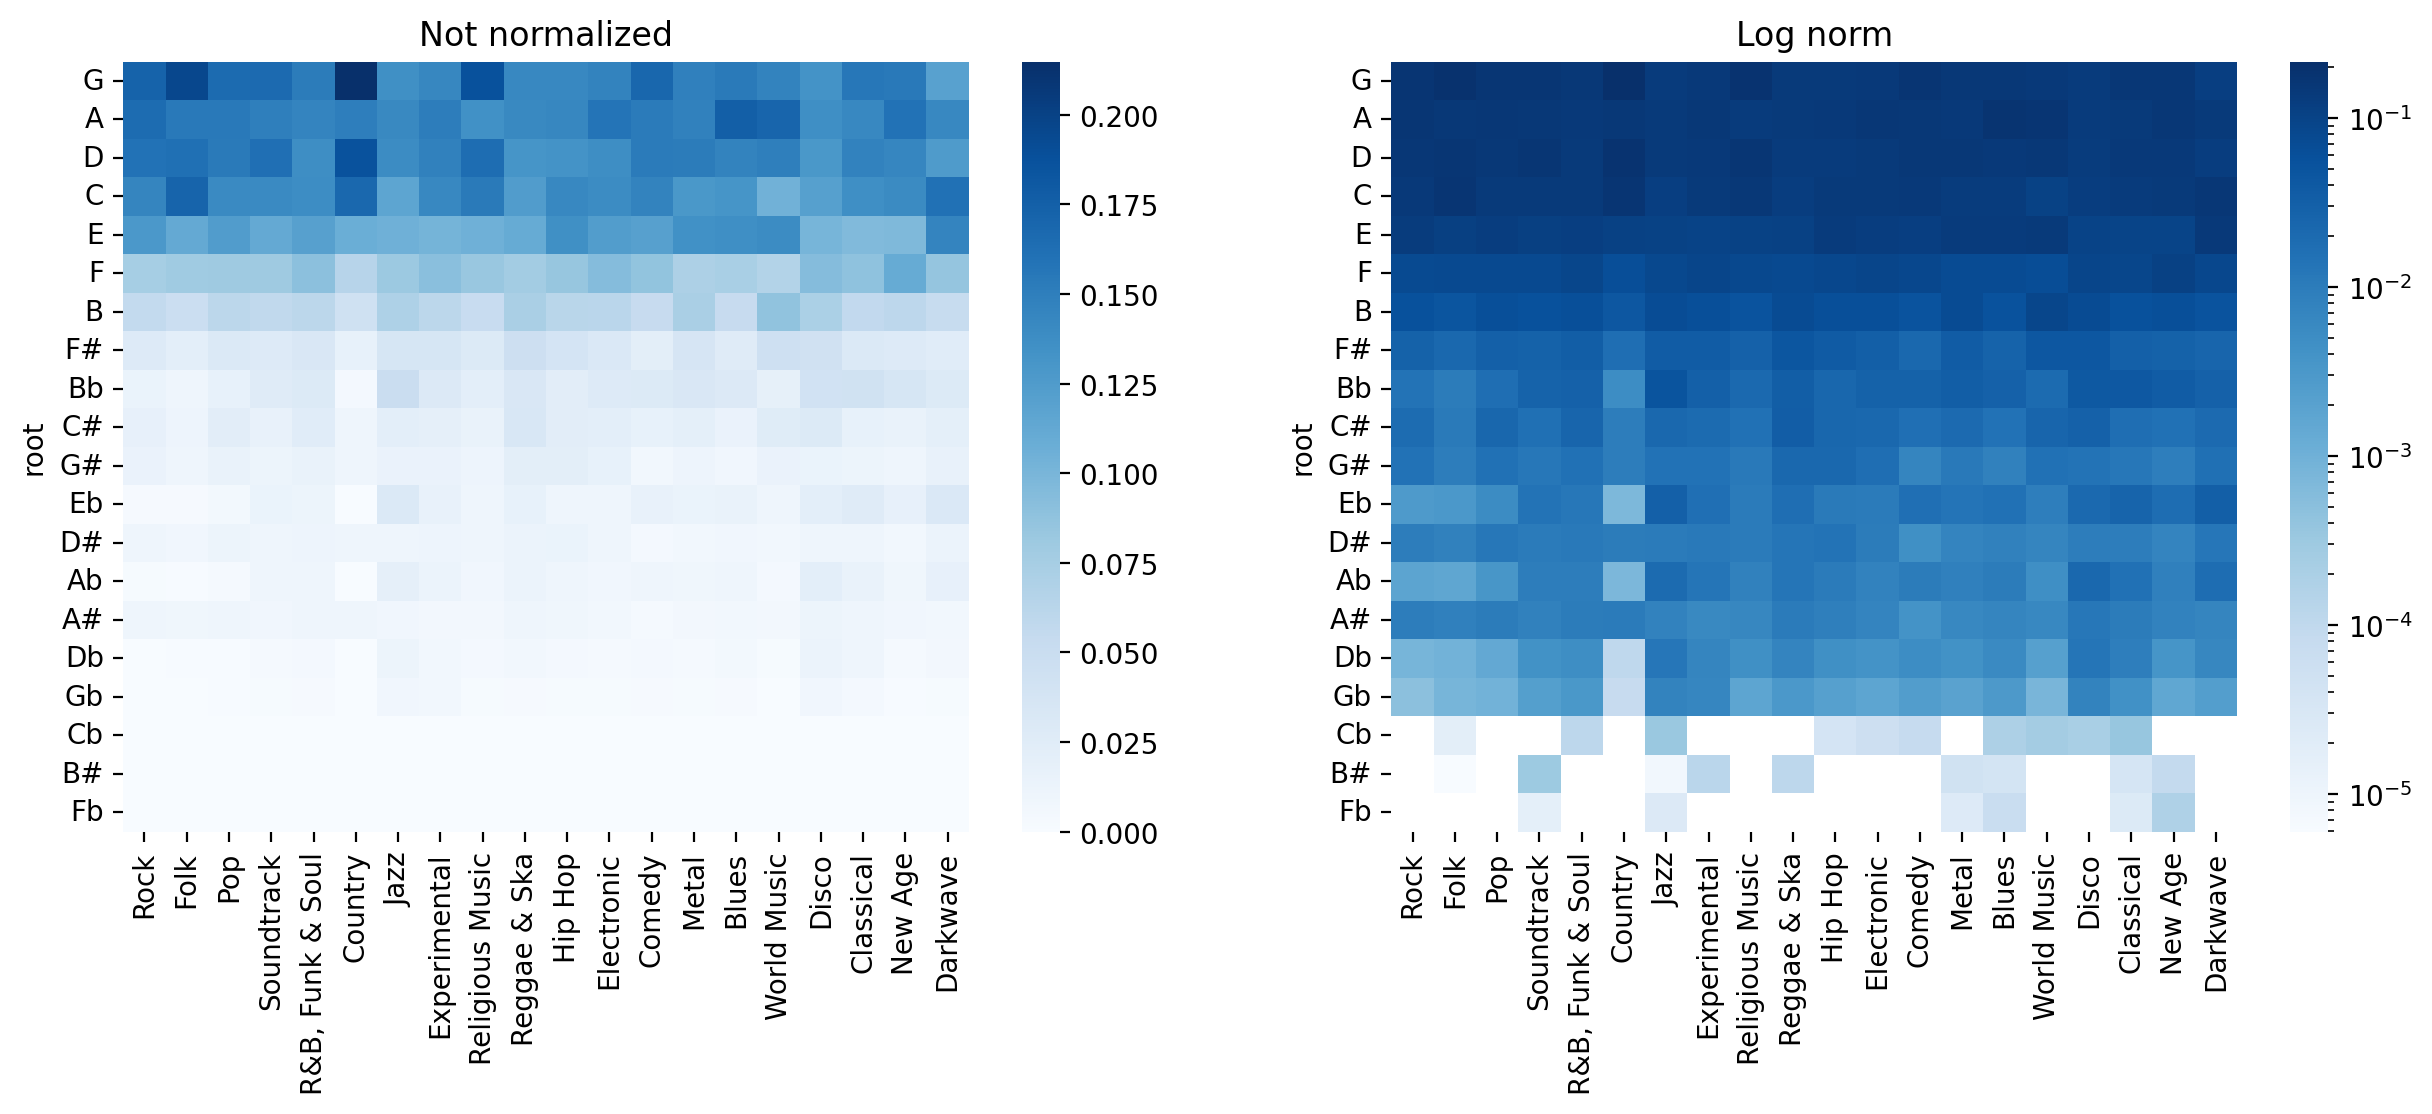
\includegraphics[width=\linewidth]{images/roots-across-genres.png}
    \end{minipage}\hfill
    \begin{minipage}{\textwidth}
        \centering
        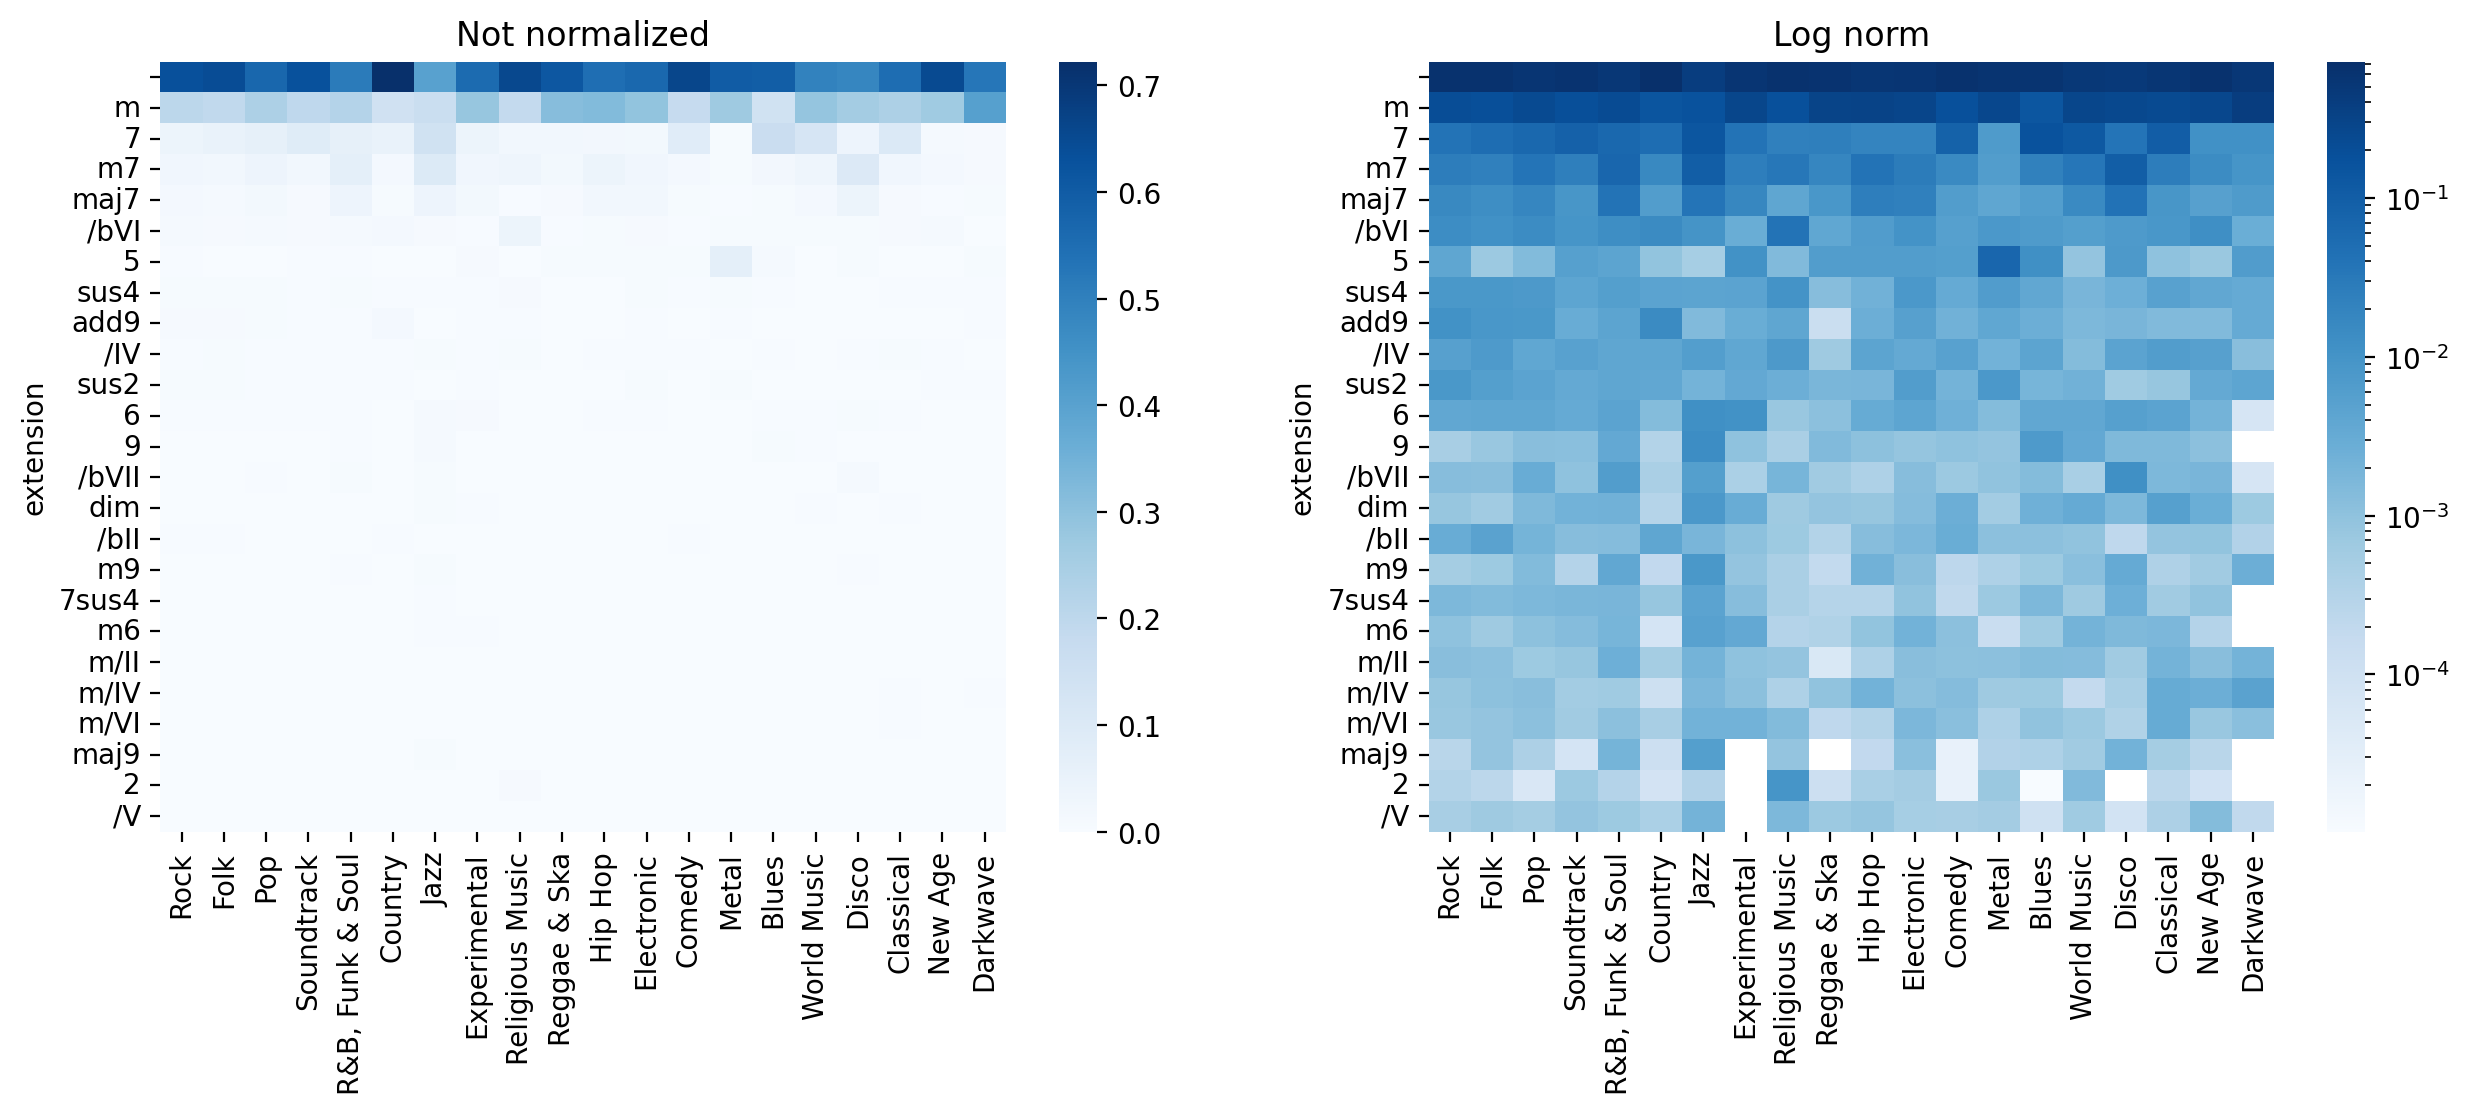
\includegraphics[width=\linewidth]{images/extensions-across-genres.png}
    \end{minipage}
    \caption{Top 25 roots and extensions across genres.}
    \label{fig:roots-extensions-across-genres}
\end{figure}

We then analyzed the chord progressions, starting with complexity. A simple metric for the complexity of the harmony can be the number of unique chords and their unique roots while treating enharmonically equivalent roots as different since the specific notation depends on the context. The overall distribution of this complexity can be found in Figure \ref{fig:num-unique-chords-roots-histogram}. Similarly, we can plot these metrics across different genres and decades (Figure \ref{fig:num-unique-chords-roots-genres-decades}). A few interesting things can be seen in the data, such as Jazz dominating in both of these metrics, while Hip Hop is the simplest. The Experimental genre has the highest variance, suggesting it contains both simple and complex forms of harmonies. An analysis over the decades shows us that the complexity of harmonies tends to grow up to around the 1970s and 1980s and decrease afterward, except for the current decade.

\begin{figure}[!htbp]
    \centering
    \begin{minipage}{.49\textwidth}
        \centering
        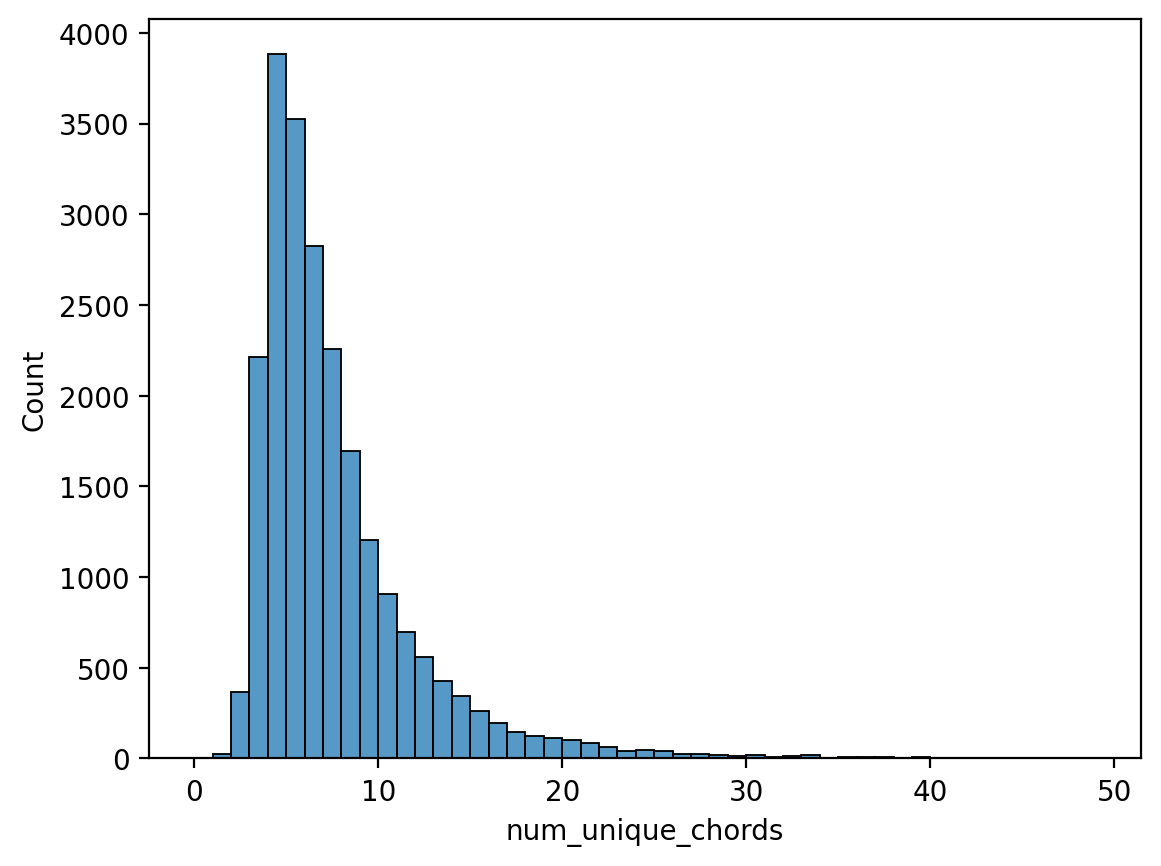
\includegraphics[width=\linewidth]{images/num-unique-chords-histogram.png}
    \end{minipage}\hfill
    \begin{minipage}{.49\textwidth}
        \centering
        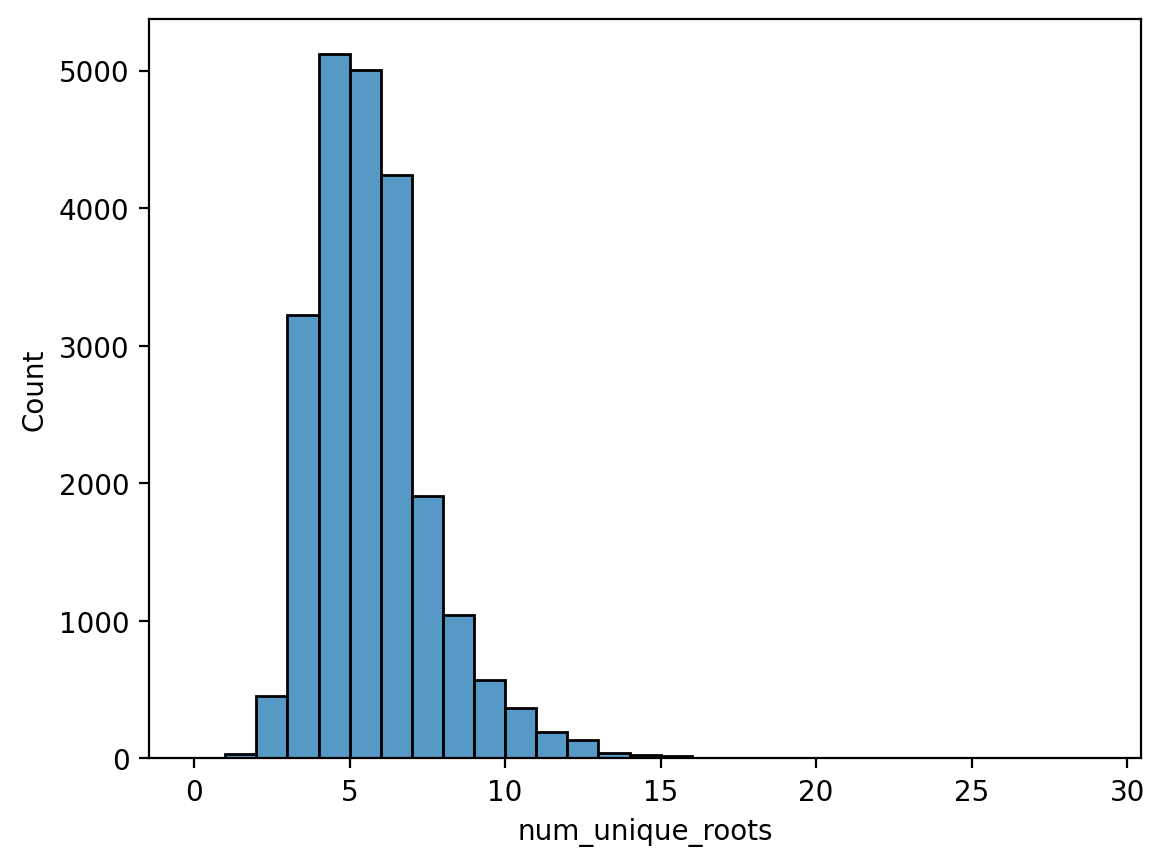
\includegraphics[width=\linewidth]{images/num-unique-roots-histogram.png}
    \end{minipage}
    \caption{Histograms of the number of unique chords and roots.}
    \label{fig:num-unique-chords-roots-histogram}
\end{figure}

\begin{figure}[!htbp]
    \centering
    \begin{minipage}{\textwidth}
        \centering
        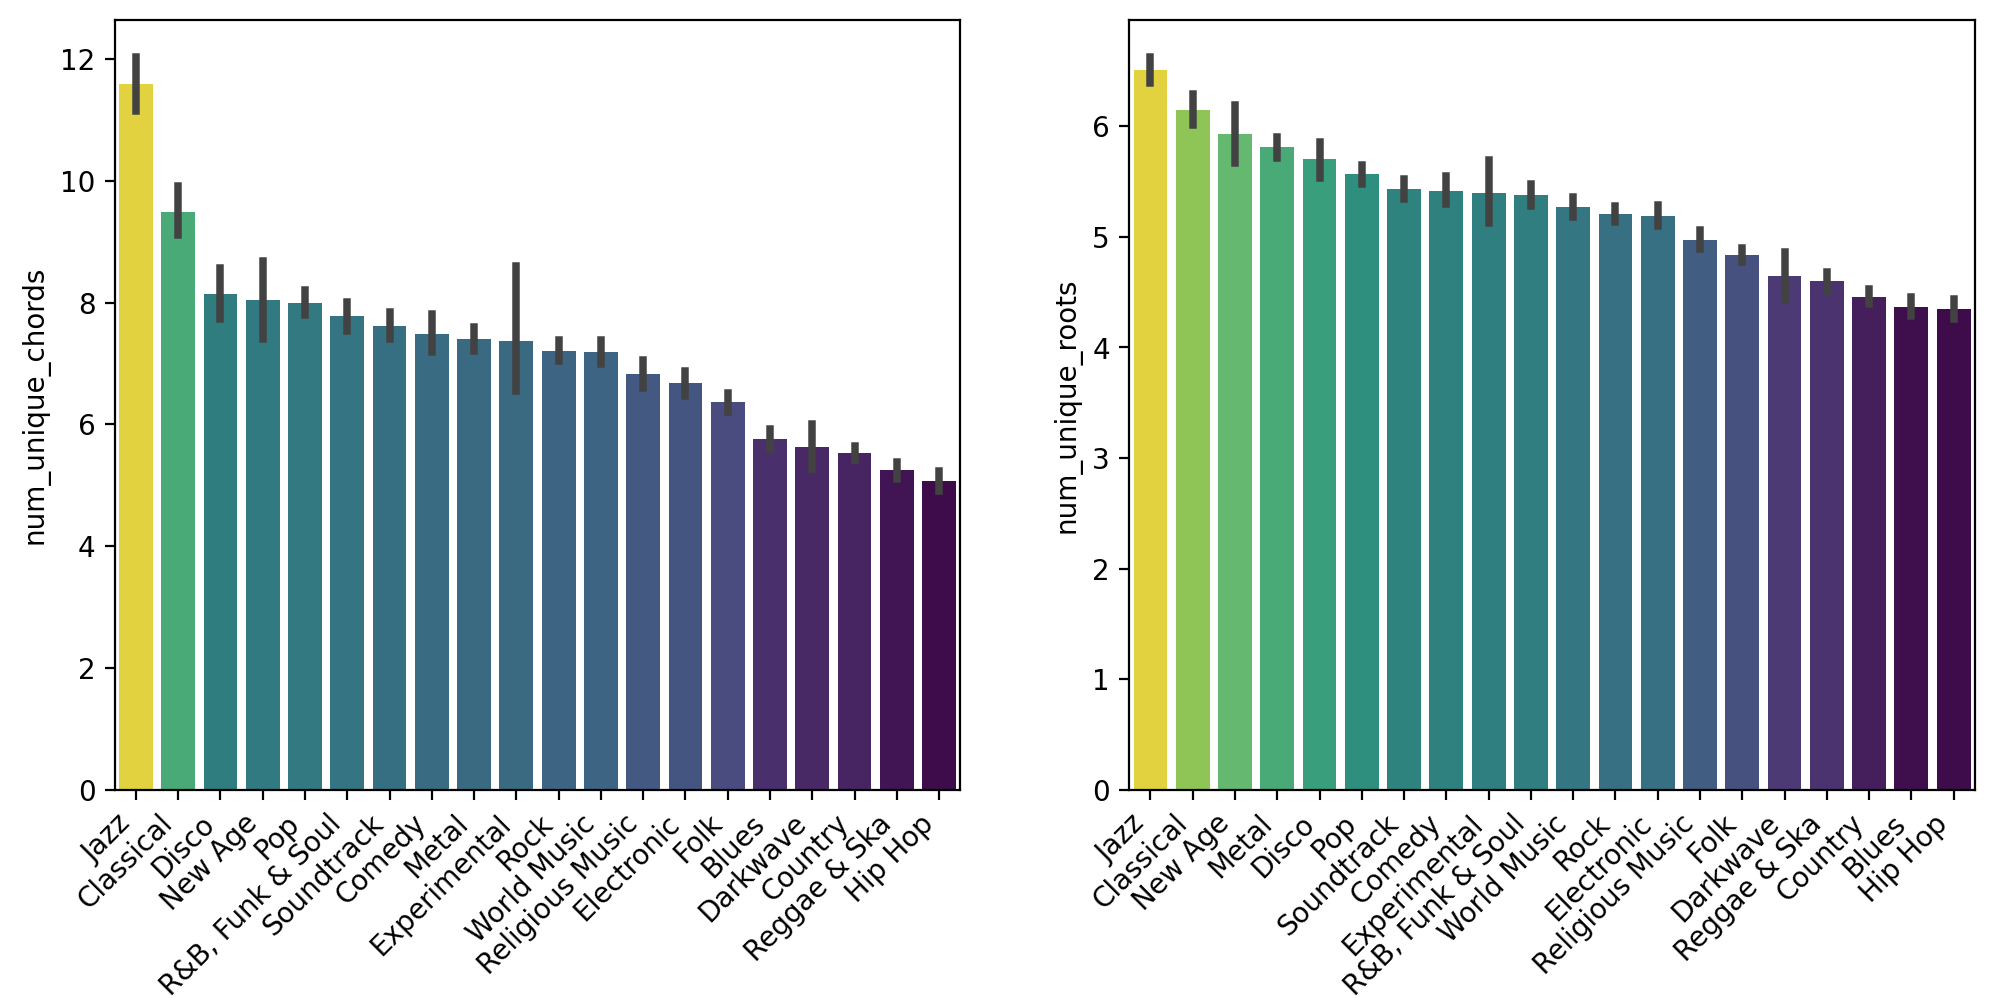
\includegraphics[width=\linewidth]{images/chords-across-genres.png}
    \end{minipage}\hfill
    \begin{minipage}{\textwidth}
        \centering
        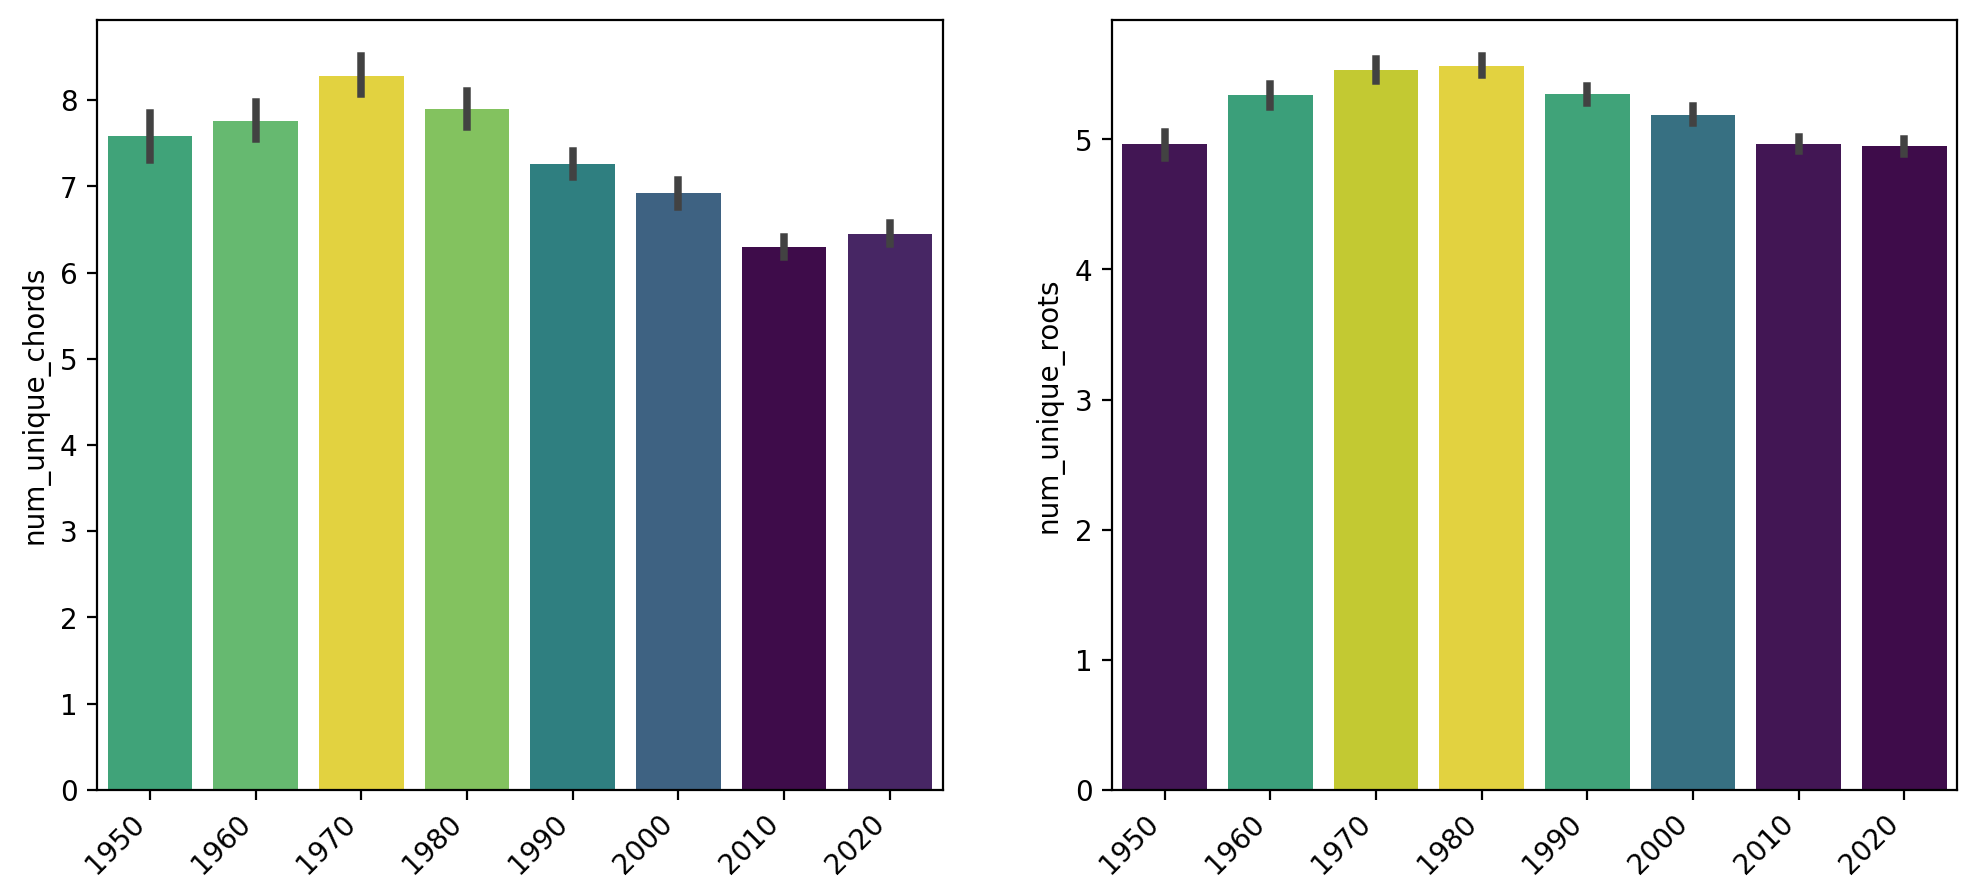
\includegraphics[width=\linewidth]{images/chords-across-decades.png}
    \end{minipage}
    \caption{Number of unique chords and roots across genres and decades}
    \label{fig:num-unique-chords-roots-genres-decades}
\end{figure}

This technique however does not take into account the complexity of the individual chords. Since measures of complexity are not strictly defined as they depend mainly on human interpretation, we attempted to create a custom metric based on the dissonance of the individual intervals forming a chord. Given the notes forming a chord, all possible pairs were compared, and the complexity scores of the individual intervals were added together and divided by the number of notes in the chord, making chords with more notes more complex by the score while maintaining a balance. The exact implementation is available on the GitHub repository.

\begin{figure}[!htbp]
    \centering
    \begin{minipage}{.49\textwidth}
        \centering
        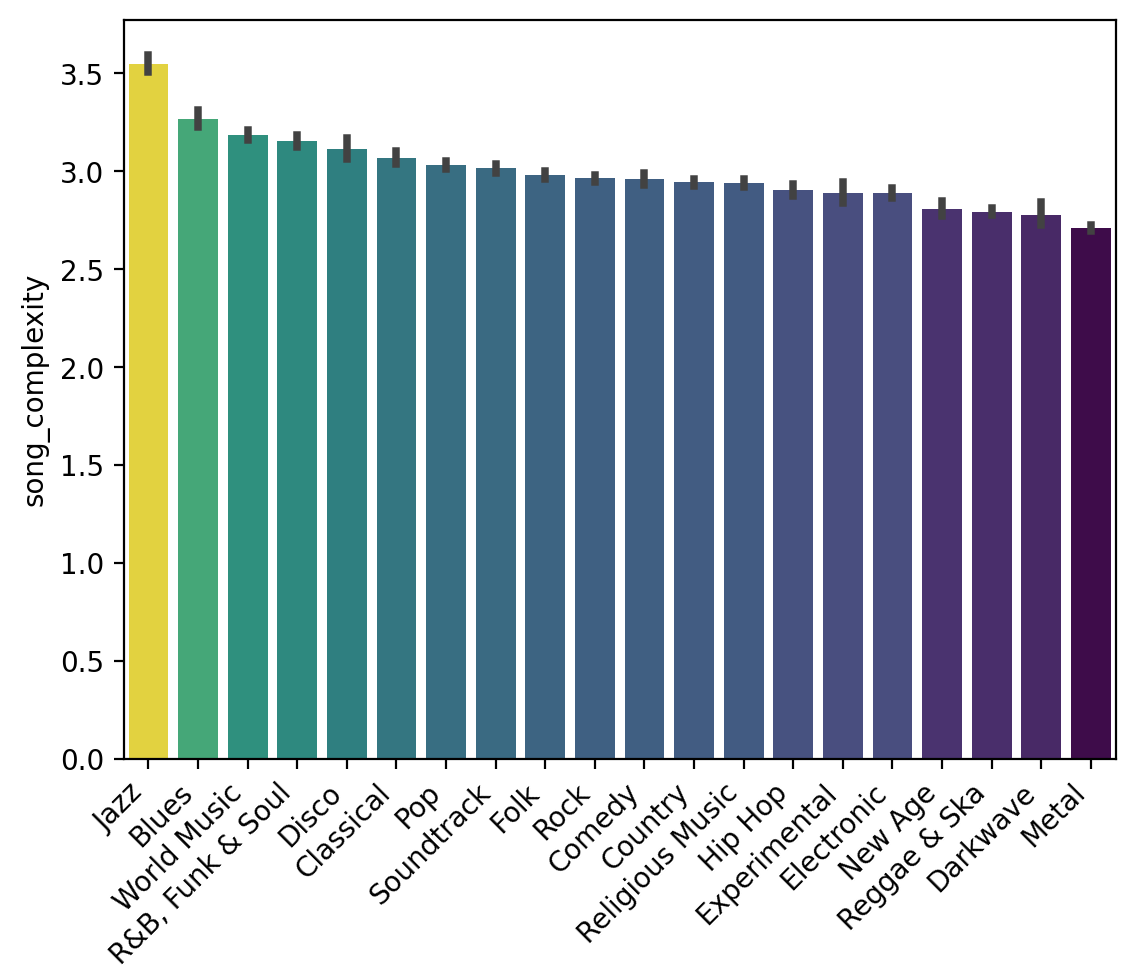
\includegraphics[width=\linewidth]{images/complexity-across-genres.png}
    \end{minipage}\hfill
    \begin{minipage}{.49\textwidth}
        \centering
        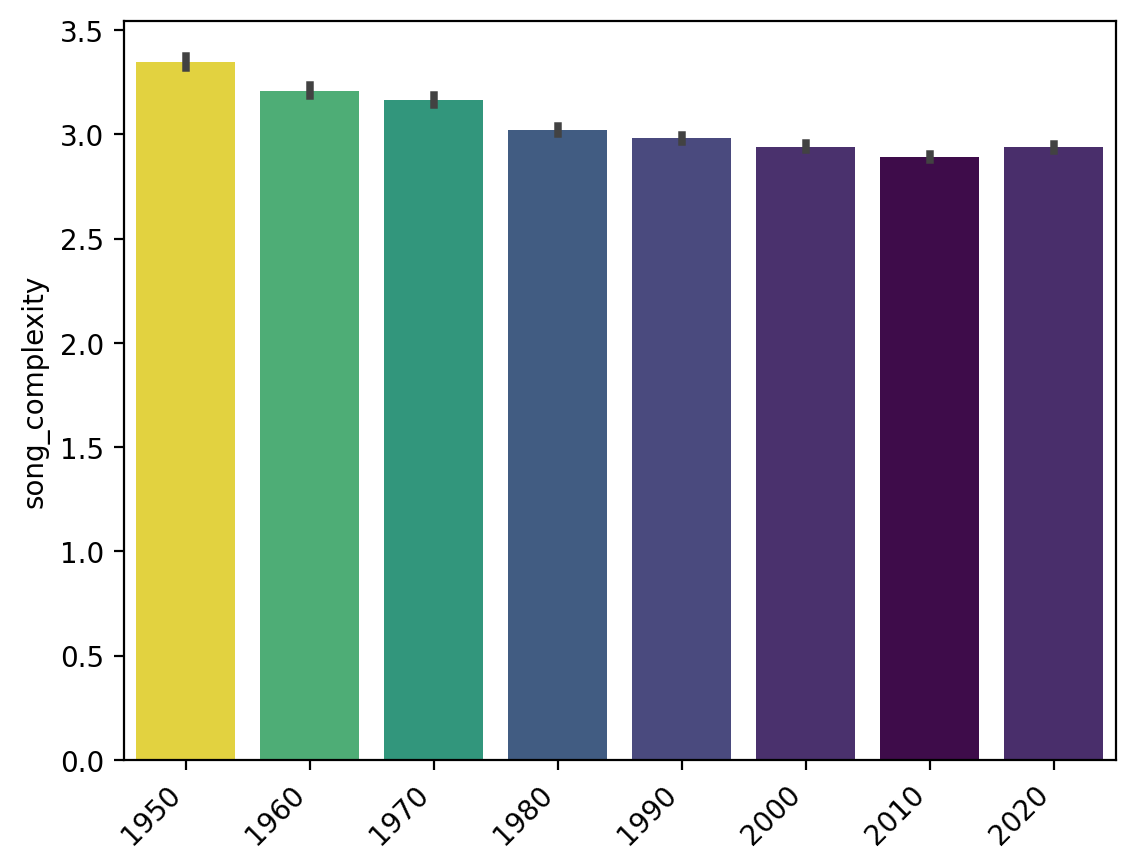
\includegraphics[width=\linewidth]{images/complexity-across-decades.png}
        \vspace{0.475cm}
    \end{minipage}
    \caption{Custom complexity score across genres and decades.}
    \label{fig:complexity-genres-decades}
\end{figure}

The average complexity of the chords used in a song was then obtained from songs across genres and decades, as depicted in Figure \ref{fig:complexity-genres-decades}. By this new metric Jazz remains the most complex genre, leaving Metal at the other end. This can be explained from the previous Figure \ref{fig:roots-extensions-across-genres}, where it is clear that Jazz uses a variety of different complex chords while Metal mostly limits itself to the use of major, minor, and power chords. Surprisingly, while Blues is quite simple given the number of unique chords and roots, this new metric places it right after Jazz. The plot over the decades shows us a bit different trend than previously, where chords tend to be less dissonant over time except for the 2020s.

To better understand the chord progressions, n-gram analysis was performed. Tonality is assumed, so Roman numerals are used to describe the chords. Note that for practical purposes, minor chords here are not denoted by lowercase letters, but by appending "m" to the uppercase variant. Since many songs use repeated chord sequences, a standard method would provide us with multiple additional n-grams (e.g. the repetition of I IV V will also produce IV V I and V I IV), therefore, a different approach was used. To treat all those different n-grams as being one, a notion of cyclic permutations and the root cyclic permutation form was introduced. Given any n-gram, the cyclic permutations of this n-gram are all the n-grams (of the same length) produced from the repetition of this n-gram. The root cyclic permutation of an n-gram is then the first of the cyclic permutations of this n-gram sorted ascendingly by the Roman numeral order; if there are multiple n-grams with the same Roman numeral order, lexicographical order is used for the non-Roman-numeric part of the chord. To focus primarily on the harmonic changes themself instead of taking into account the broader context, the n-gram is also normalized to make the lowest Roman numeral always I. Note that this process can produce n-grams starting with I I, which may look like a mistake since consecutive chords were removed, which can be explained by realizing that a sequence like I IV V I gets normalized to the n-gram I I IV V. Although this procedure may seem complex, it gives us easily interpretable results.

\begin{figure}[!htbp]
    \centering
    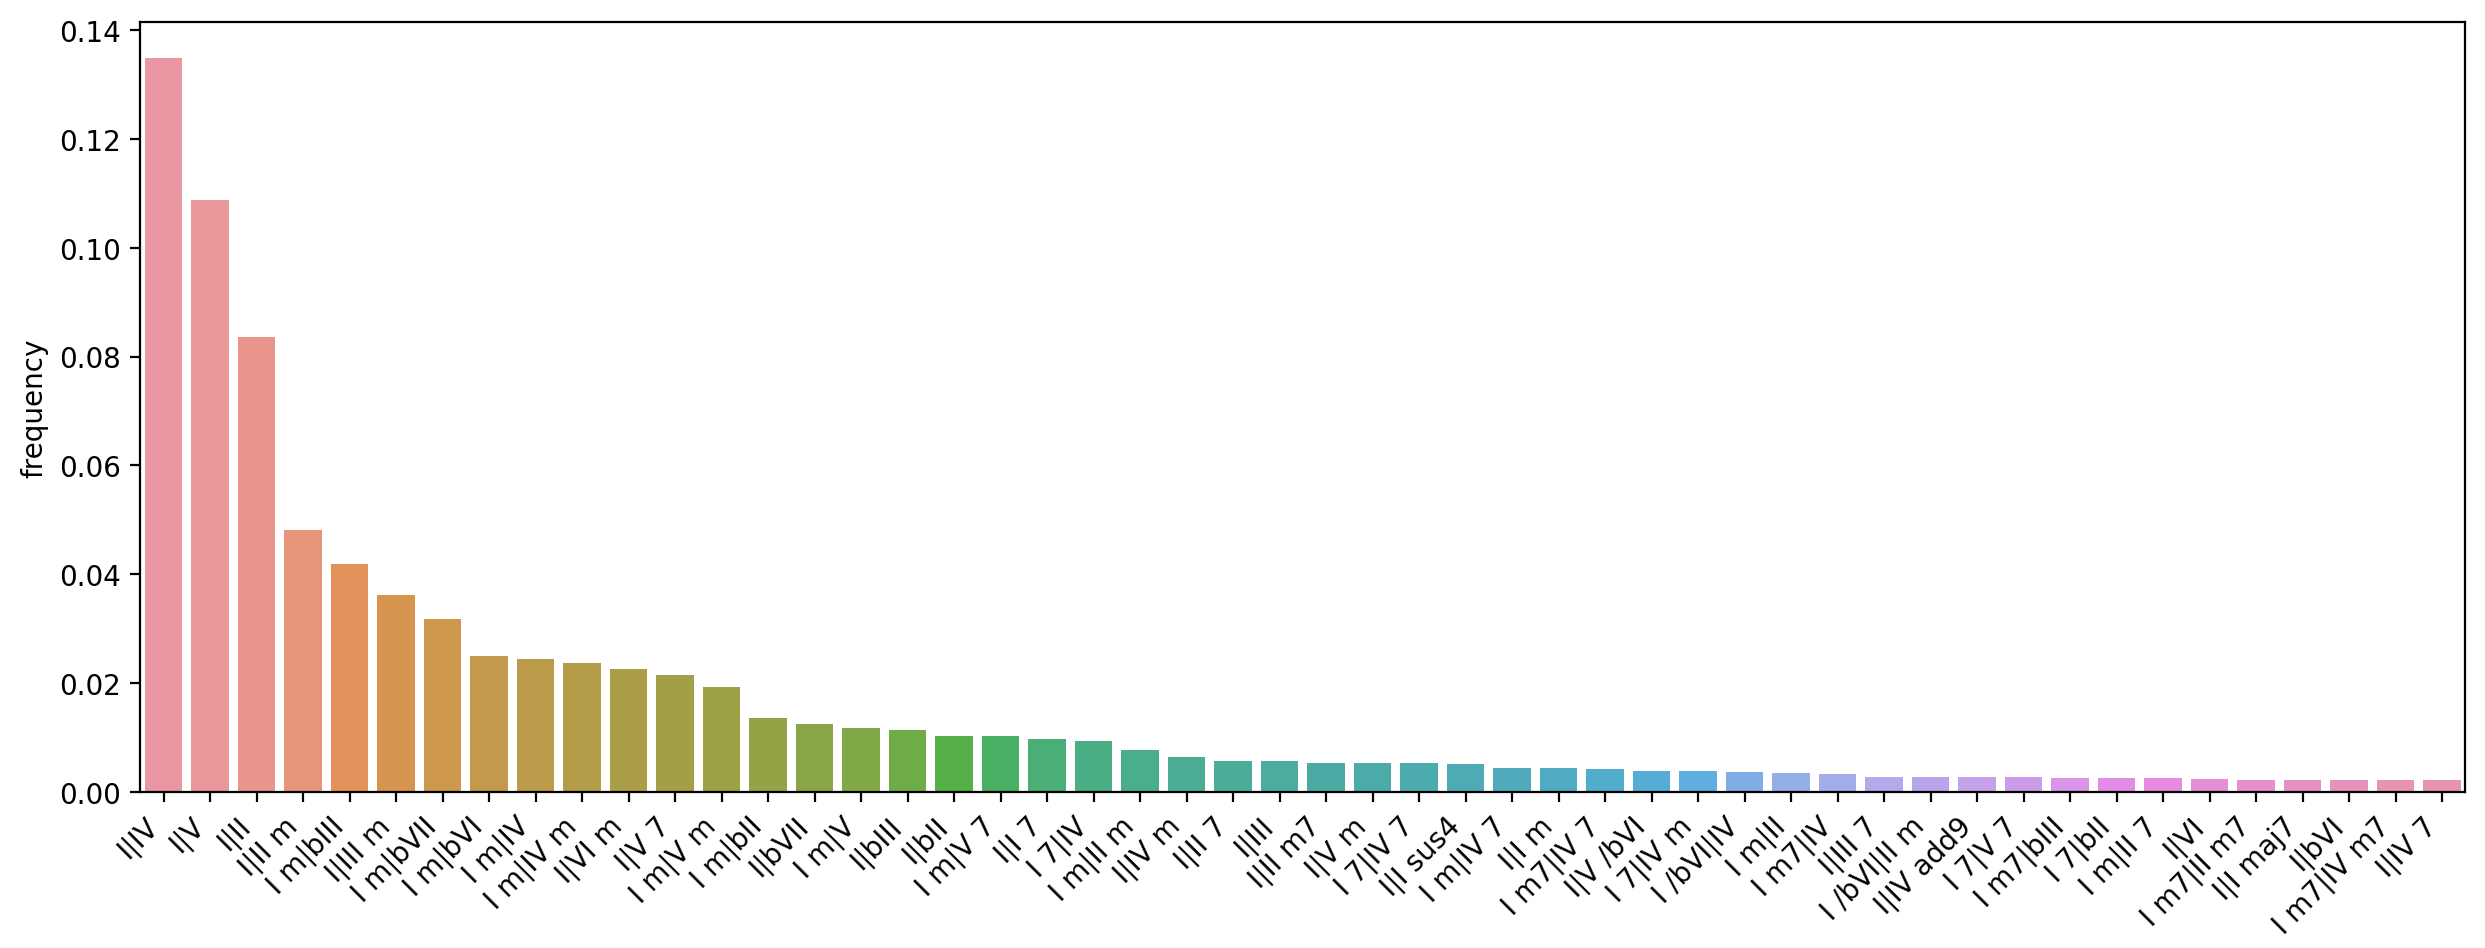
\includegraphics[width=\linewidth]{images/bigram-plot.png}
    \caption{Top 50 bigrams.}
    \label{fig:bigram-plot}
\end{figure}

\begin{figure}[!htbp]
    \centering
    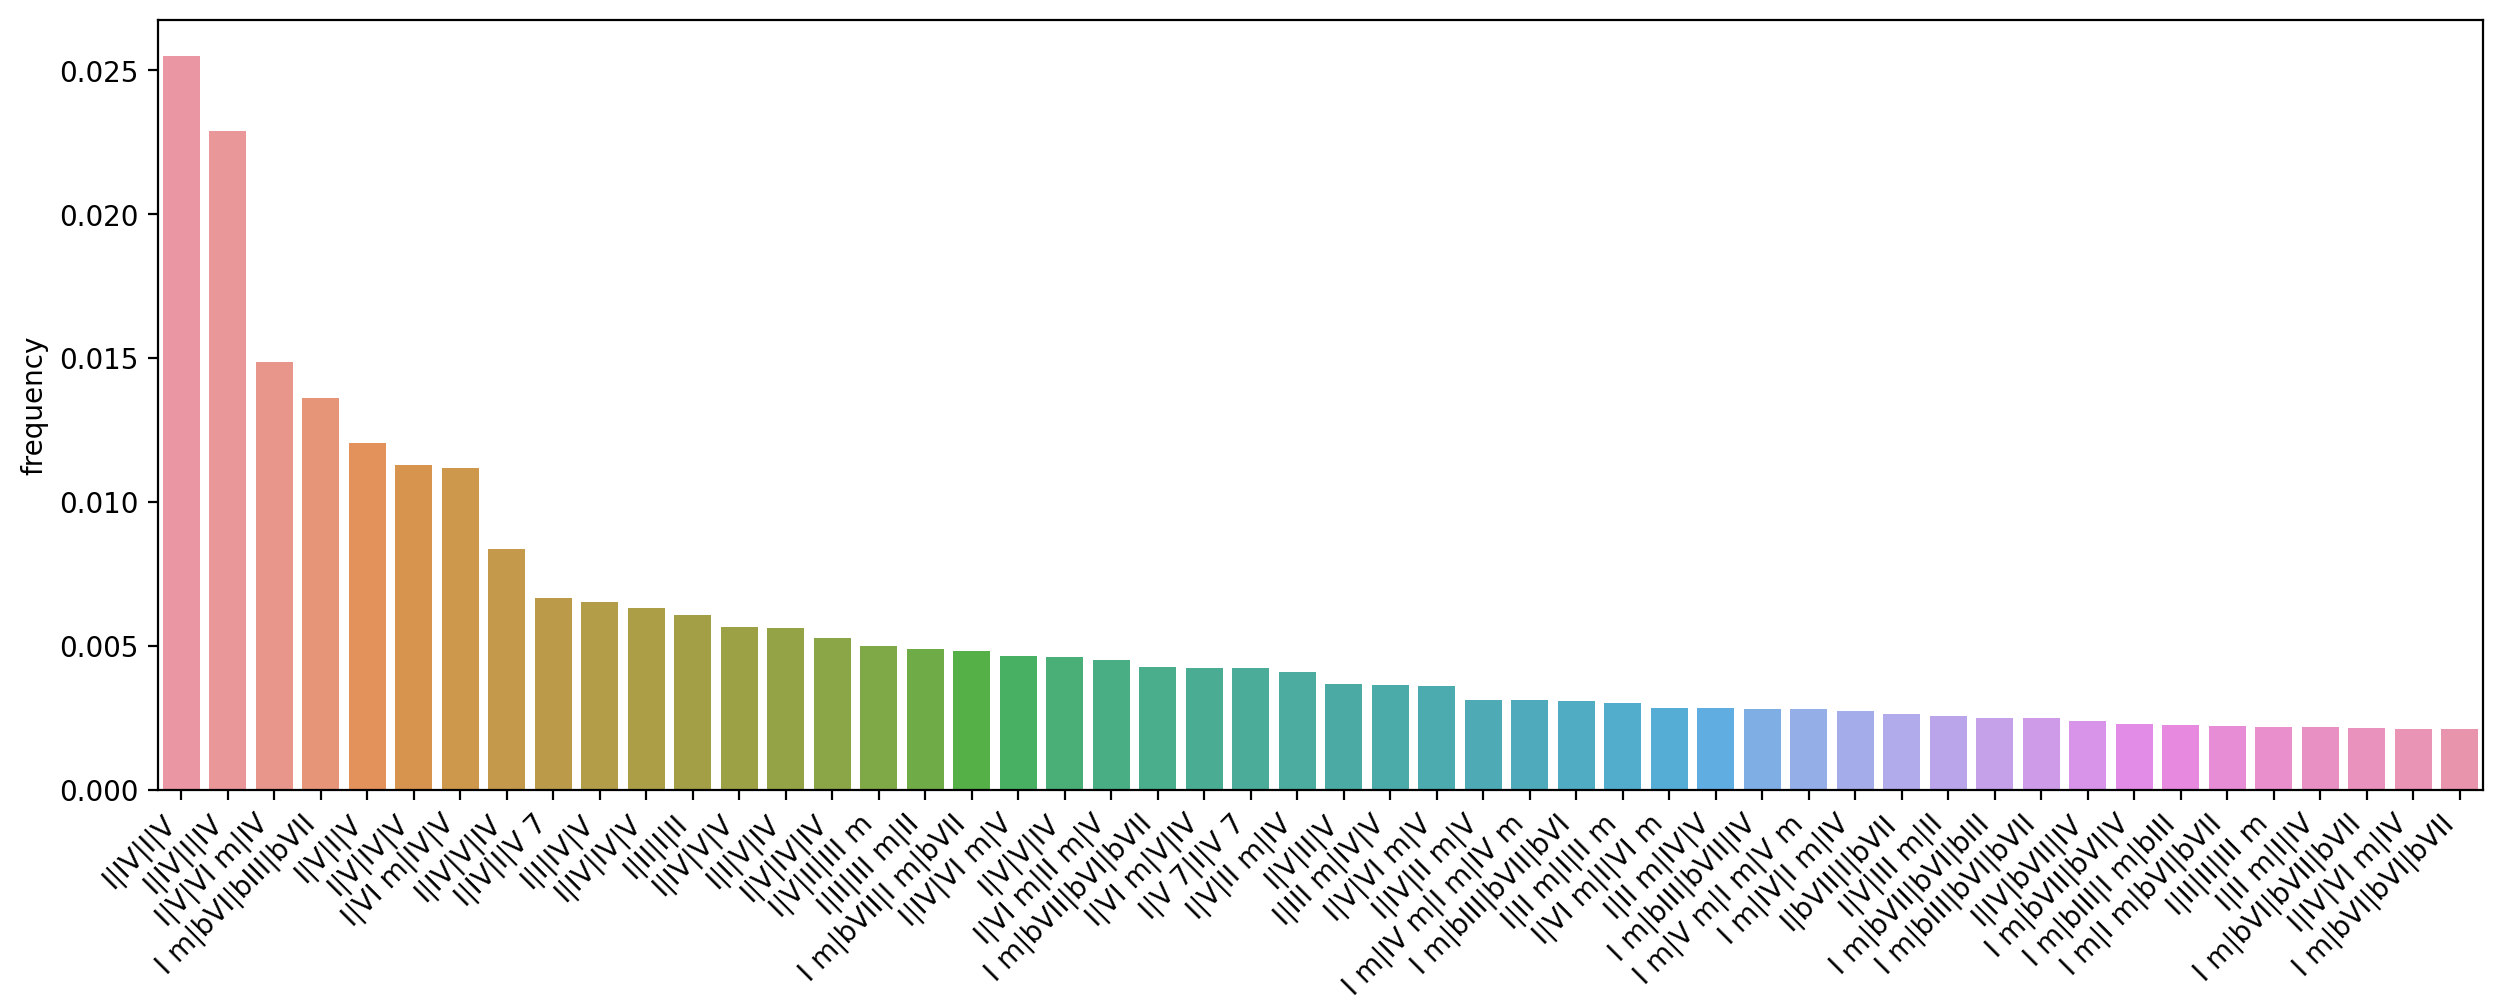
\includegraphics[width=\linewidth]{images/fourgram-plot.png}
    \caption{Top 50 fourgrams.}
    \label{fig:fourgram-plot}
\end{figure}

In the Figures \ref{fig:bigram-plot} and \ref{fig:fourgram-plot}, the top 50 bigrams and fourgrams are shown. Frequency represents the proportional distribution of the n-gram (normalized and converted into the root cyclic permutation) in the whole dataset. The form of the chord is separated from the Roman numeral by a space, the chords are then separated by a vertical bar. Similar plots were also created for the top four genres, Jazz and Metal (as our previous metric puts these into the opposite ends of the complexity spectrum), they can be found with the full exploratory data analysis on GitHub.

\subsection{Data Tokenization} \label{Data Tokenization}

Our dataset contains a large collection of different chords where many synonyms exist, formed not only by enharmonically equivalent notes but also by different chord notations used. The music21 library \cite{music21} allows us to parse a variety of different chords, however, for our purposes, this method is very limited as it fails on a significant portion of the data. There is not a broad publicly available algorithm for parsing chord symbols, as its creation is not trivial. Thanks to the way the data was scraped, we have a map of 4,986 chord symbols to note after transposing them to all possible keys. When merging synonyms by the notes used, we get just 3360 tokens. However, this number is still too large given the size of our dataset to be usable. Instead, a new method for synonyms had to be developed.

\begin{figure}[!htbp]
    \centering
    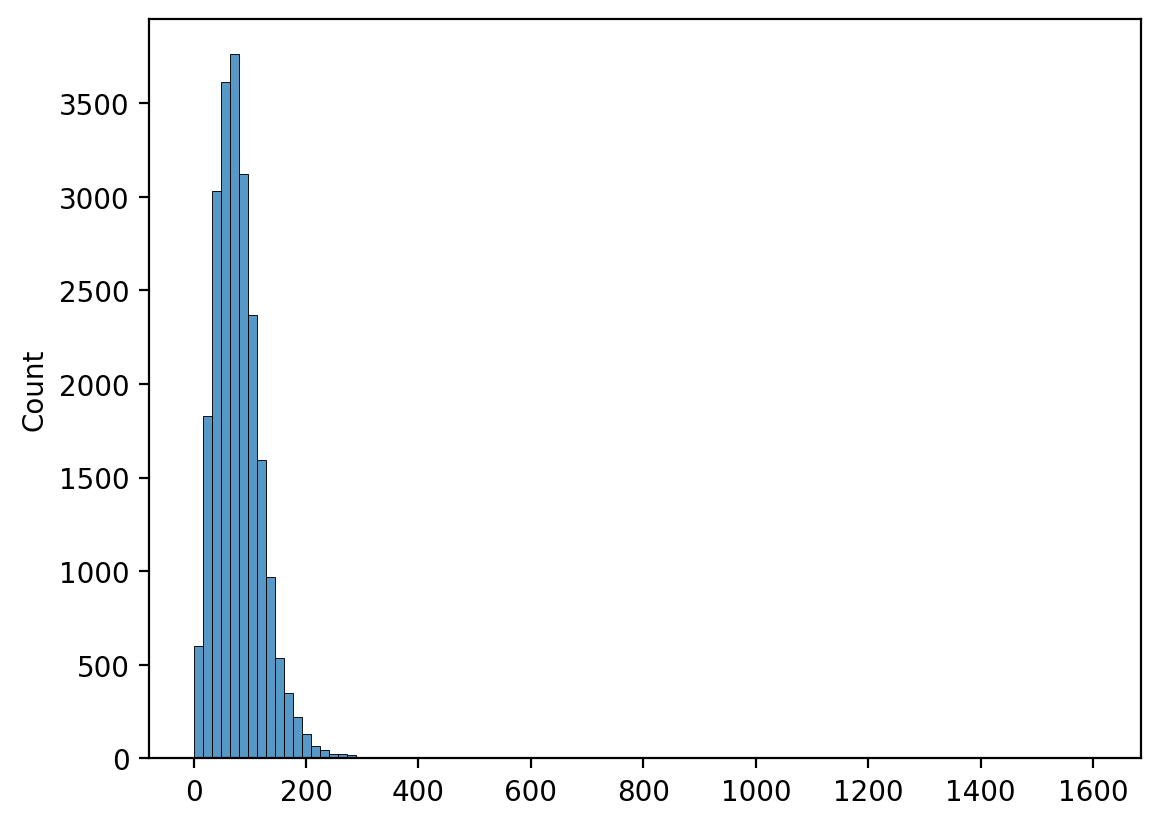
\includegraphics[width=0.7\linewidth]{images/chord-sequence-lengths.png}
    \caption{Histogram of sequence lengths.}
    \label{fig:chord-sequence-lengths}
\end{figure}

Ideally, we would want to treat the inversions of individual chords as the same chord, since just changing the inversion of a chord does not make an important change to its function. It would be important if we also wanted to incorporate chord voicings, but for such purposes, a different dataset would be more suitable (such as one constructed from MIDI samples), thus we leave it as a matter of future work. One important aspect of chord inversions and other voicing methods is that the pitches used remain the same when they are all transposed to the same octave. This idea can be used to construct pitch class tokenization, where we process each chord as a binary vector of twelve elements and assign a token to each new unique representation. With this approach, the theoretical upper limit of tokens is $2^{12}=4,096$, but for practical purposes, we will use only representations that are present in the dataset, leaving us with only 1,033 tokens. In practice, another two extra will be used, namely, the start and end of sequence tokens. 

After tokenizing the data in this way, all sequences with more than 256 tokens (including the start and end of sequence tokens) were dropped. From Figure \ref{fig:chord-sequence-lengths}, we can see that this is sufficient to cover most of the sequences. This step is required to train the models efficiently since the lengths of individual sequences inside a mini-batch must be the same (padding will be used to fill in the extra spaces).

\section{Model Development}

\subsection{Evaluation Metrics}

Before discussing the architectures used to model the data, we introduce a few metrics to properly describe their performance, as the evaluation of generative models is not trivial. In section \ref{Human Evaluation}, we will discuss human evaluation, as it is often the only way to get a somewhat objective measure of performance that can be compared with other techniques.

\textbf{Top-1 Accuracy.} Given raw prediction outputs, the portion of the time the top prediction matches the real token. An easily interpretable metric, limited by ignoring the other predictions, even though their value is also important. We will also refer to this metric as just the accuracy.

\textbf{Perplexity.} Defined as the exponentiation of the entropy of the probability distribution; in other words, the inverse model-predicted probability of a reference sequence of tokens, normalized by the number of words. Intuitively can be thought of as a measure of how "surprised" the model is by the data. We will compute both accuracy and this metric on the original datasets, without applying augmentation. Lower values indicate better performance.

\textbf{Fr\'echet Feature Distance.} Fr\'echet Inception Distance (FID) is a common metric used to describe the performance of image generative networks. It compares the distributions of the extracted features (using the InceptionV3 model, hence the name) of real and generated samples. A similar approach was used for our task, where a classifier Transformer network was trained to predict the genre and decade of a sample to act as a feature extractor. Its architecture was almost the same as the large variant of our generative Transformer, described in section \ref{Transformer}, except for the output layer. The values from the last layer before the output layer were averaged across the token dimension, leaving us with a 96-dimensional feature vector. The Fr\'echet Feature Distance (FFD) was then obtained by comparing the feature vectors of the test samples with the same number of generated samples. This metric is limited in a few ways, such as that its value tends to decrease with the number of samples used, but provides a better idea of the distribution of the samples the model generates. The scores are only reported on the augmented test set, as we want the generated samples to be of all the possible keys. Lower values indicate better performance.

We also tried to develop a few other metrics, such as those comparing the distribution of n-grams across the generated and real sequences using cosine similarity and Fr\'echet distance, but they were mostly unsuccessful due to not being descriptive enough or memory and compute limitations.

\subsection{Recurrent Network}

Since recurrent architecture is the backbone of many popular generative music architectures, we created a simple gated recurrent network to establish a reference performance for other, more sophisticated architectures. The hyperparameters are chosen to strike a balance between performance and compute, training a larger variant with the same overall structure resulted in insignificant changes in the performance.

The architecture is structured as follows:

\begin{itemize}
    \item \textbf{Embedding Layer}: Maps the input into a 96-dimensional embedding space. 
    \begin{itemize}
        \item \textit{Input}: A sequence of tokens
        \item \textit{Output}: 96-dimensional embeddings
    \end{itemize}
    
    \item \textbf{GRU Layers}: A three-layer gated recurrent unit (GRU) with 96 units.
    \begin{itemize}
        \item \textit{Input}: 96-dimensional embeddings from the previous layer
        \item \textit{Output}: 96-dimensional GRU output
    \end{itemize}

    \item \textbf{Multilayer Perceptron (MLP)}: A sequence of linear transformations and non-linear activations.
    \begin{itemize}
        \item \textit{Layers}: 
        \begin{enumerate}
            \item Linear layer (96 to 96 units)
            \item ReLU activation
            \item Linear layer (96 to the size of the vocabulary units)
        \end{enumerate}
        \item \textit{Output}: Final output of the vocabulary size.
    \end{itemize}

    Total number of parameters: $376,683$
\end{itemize}

The dataset was split into a train set and a test set, in an 80/20\% split to make the test set representative of the overall distribution. During training, a batch size of 128 samples was used. To artificially increase the dataset size, transposition was employed to train on sequences in random keys. In addition, it also makes the model invariant to the key used. Another common method is to transpose all the sequences into the same key and train the model on it instead \cite{DBLP:journals/corr/abs-1709-01620}, however, we did not use this approach as obtaining the proper key is non-trivial (one cannot just pick the tonality of the first chord) and it would not account for modulation (possibly treating modulated parts differently and obtaining worse performance on such samples).

Since we were training on padded data, a masking mechanism was developed for the cross-entropy loss and top-1 accuracy calculation. The Adam optimizer was used with a 0.001 initial learning rate ($\beta_1=0.9, \beta_2=0.999$), with a learning rate scheduler multiplying it by 0.3 every 10 epochs. The model was trained for 50 epochs, allowing convergence to occur. The embedding layer was trained from scratch, as using popular word embedding techniques for the chords made the convergence only insignificantly faster.

The model achieved $56.00\%$ top-1 accuracy on the train set and $56.59\%$ on the test set. The final perplexity was $4.927$ on the train set and $4.851$ on the test set. Given our FFD metric, the model scored $9.290$. These metrics suggest that the model is underfitting the training data, however, as discussed earlier, increasing the model size did not make significant changes, so a different architecture was used to achieve better results.

\subsection{Transformer} \label{Transformer}

The Transformer architecture has recently seen massive success in language modeling, especially with the dawn of large language models \cite{brown2020language, JMLR:v24:22-1144, touvron2023llama, workshop2023bloom}. It has been shown that it is superior to recurrent networks, thanks to relying solely on the attention mechanism, allowing better parallelization, training efficiency, and global dependencies while achieving better performance \cite{NIPS2017_3f5ee243}. The global attention mechanism can intuitively help in music-related tasks, as it enables the model to understand complex patterns over long sequences, which is crucial in music composition. Since we are dealing with discrete sequences of tokens, we can easily apply the (decoder-only) Transformer architecture for our task.

Three distinct model sizes were developed: TransformerS, TransformerM, and TransformerL, representing small, medium, and large sizes, respectively. Each model is based on a standard decoder-only Transformer architecture, with varying specifications as detailed in Table \ref{tab:transformer_specs}. The maximum sequence length is constant at 256 tokens among the models, as described in Section \ref{Data Tokenization}.

\begin{table}[!htbp]
    \centering
    \begin{tabular}{lccc}
        \toprule
        Feature & TransformerS & TransformerM & TransformerL \\
        \midrule
        Embedding Dimension (\(d_{\text{model}}\)) & 64 & 80 & 96 \\
        Number of Heads (\(n_{\text{heads}}\)) & 8 & 10 & 12 \\
        Number of Transformer Layers (\(n_{\text{layers}}\)) & 6 & 12 & 24 \\
        Total Number of Parameters & 433,419 & 1,100,715 & 2,883,915 \\
        \bottomrule
    \end{tabular}
    \caption{Specifications of Transformer Models.}
    \label{tab:transformer_specs}
\end{table}

The same data split and training hyperparameters were used as for the recurrent network, as they were shown to be robust enough.

\begin{table}[!htbp]
    \centering
    \begin{tabular}{lrrrrr}
        \toprule
        Model & Train Perplexity & Test Perplexity & Train Accuracy & Test Accuracy & FFD \\
        \midrule
        TransformerS & 3.157 & 3.123 & 68.74\% & 69.05\% & 3.201 \\
        TransformerM & 2.682 & 2.677 & 73.77\% & 73.91\% & 2.814 \\
        TransformerL & 2.506 & 2.513 & 75.98\% & 76.04\% & 2.316 \\
        \bottomrule
    \end{tabular}
    \caption{Performance of Transformer models.}
    \label{tab:transformer_performance}
\end{table}

The performance metrics are shown in Table \ref{tab:transformer_performance}. We can see a significant improvement compared to the recurrent architecture, even with the small variant. The performance improves with model size, but it seems to start to plateau with the largest variant. Since we can see practically the same performance on both the train and test sets, it suggests that we have not overfitted and could scale the models further without needing more data.

\subsection{Conditional Transformer}

One important aspect of generative deep learning is the controllability of the process. Some standard methods include conditional generation, where a certain condition, such as the genre of a song, is used in addition to the sequence data; and style-based approaches, which generate based on an unentangled latent space, which can be easily explored, as is the case with modern generative adversarial networks (GANs).

Naively, one could think that simply adding an extra "style" token to the start of the sequence for the Transformer architecture would enable it to generate in regards to that style. However, empirically it seems that this approach results in the final model just ignoring the additional style information, as we have unsuccessfully tried this method. A more sophisticated approach had to be developed, that would enforce the model to use styling nonetheless. We took inspiration from the StyleGAN architecture \cite{karras2019stylebased}, which, among others, uses adaptive instance normalization to control the generation process, and applied a similar technique to our objective.

Since we are dealing with the Transformer architecture that uses layer normalization, we will modify all of those occurrences into adaptive layer normalization. Let $x \in \mathbb{R}^{sequence\_length \times d_{model}}$ be some hidden representation and $w \in \mathbb{R}^{d_{model}}$ a vector denoting the style of the sequence. Then, we specialize the $w$ into $\phi=(\phi_g, \phi_b)$ using a learnable non-linear transformation (in our case, a ReLU function followed by a linear layer is used), such that $\phi_g, \phi_b \in \mathbb{R}^{d_{model}}$. We also repeat $\phi_g, \phi_b$ along the first dimension to get them into shape $sequence\_length \times d_{model}$. The adaptive layer normalization is then 
\begin{equation}
    \mathrm{AdaLN}(x, \phi) = (1 + \phi_g) * \mathrm{LayerNorm}(x) + \phi_b,
\end{equation}
where $\mathrm{LayerNorm}$ is the layer normalization, as implemented in PyTorch. This results in an element-wise affine transformation of the normalized hidden representation $x$.

\begin{figure}[!htbp]
    \centering
    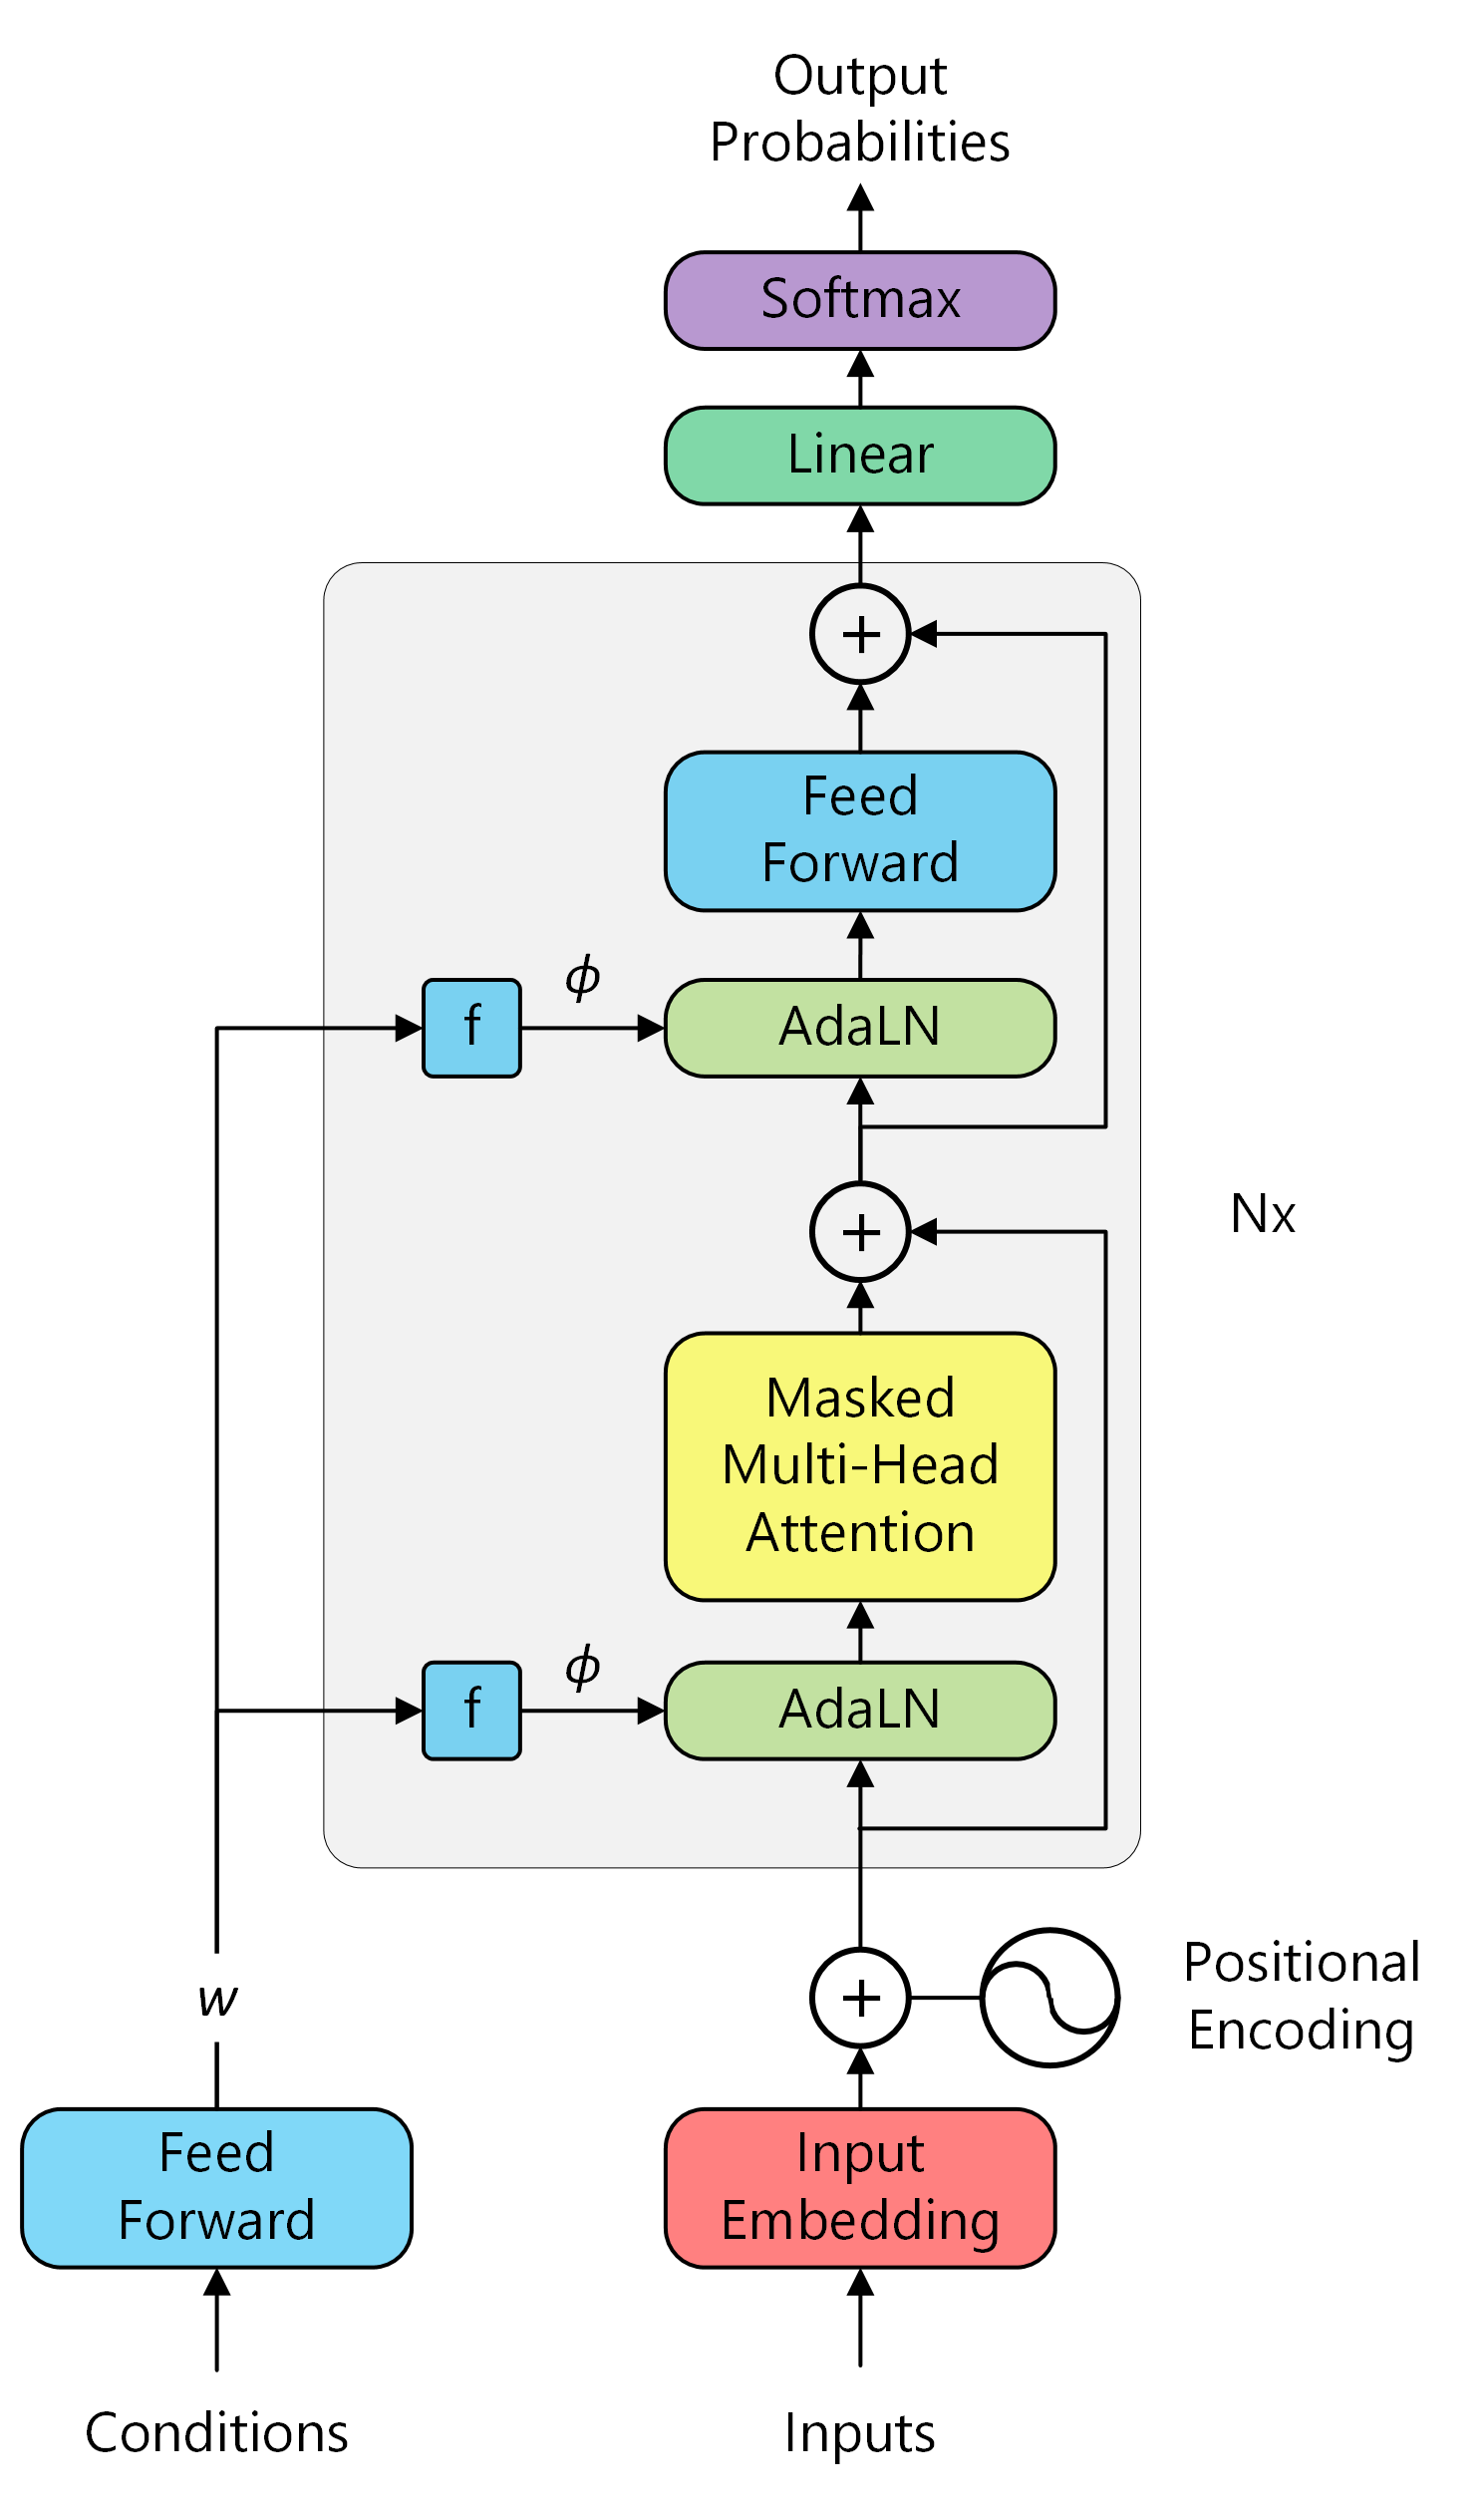
\includegraphics[width=0.35\linewidth]{images/conditional-transformer.png}
    \caption{The Conditional Transformer.}
    \label{fig:conditional_transformer}
\end{figure}

In the case of the Conditional Transformer, we take the genre and decade of the sequence and represent it as a vector. Since multiple genres can be associated with a sequence, we equally distribute the weight among them so that the weights sum to one. The final conditional vector is obtained from the concatenation of the genre vector and one-hot decade vector. We then use a learnable linear transformation to get it to the desired shape and use it as the vector $w$ in all of the adaptive layer normalization.

This approach allows each layer to influence the hidden representation based on the genre and decade independently and uniquely. $1 + \phi_g$ is used instead of just $\phi_g$ to approximately match an identity function, as we expect $\phi_g$ to have a mean of zero. An element-wise transformation is used instead of a global one to encourage specific aspects of the hidden state, similarly as some feature maps are boosted relative to each other in the StyleGAN architecture. A more efficient way to drive the styling could be developed, but we leave this for future work.

As with the Transformer architecture, three distinct sizes with the same hyperparameters as previously were developed. The total number of parameters was $535,115$ for the small variant, $1,414,075$ for the medium, and $3,780,651$ for the large one. Training and data processing were done in the same way as previously, except that the large variant was trained with a batch size of 96 samples due to memory constraints.

To calculate the FFD, the model had to generate sequences based on the genres and decades, so they were sampled from the train set distribution.

\begin{table}[!htbp]
    \centering
    \begin{tabular}{lrrrrr}
        \toprule
        Model & Train Perplexity & Test Perplexity & Train Accuracy & Test Accuracy & FFD \\
        \midrule
        ConditionalS & 3.548 & 3.521 & 64.58\% & 64.81\% & 2.998 \\
        ConditionalM & 2.785 & 2.774 & 72.75\% & 72.99\% & 2.076 \\
        ConditionalL & 2.551 & 2.562 & 75.14\% & 75.14\% & 1.848 \\
        \bottomrule
    \end{tabular}
    \caption{Performance of Conditional Transformer models.}
    \label{tab:conditional_transformer_performance}
\end{table}

In Table \ref{tab:conditional_transformer_performance}, we can see that while the perplexity and accuracy scores are a bit worse than the Transformer network (especially with the smaller variants), the FFD was improved. This may suggest that the way we enforce the condition is too strict, as it hurts the prediction capabilities of the model while improving the diversity of the samples.

\subsection{Style Transformer} \label{Style Transformer}

The improvement of FFD with the Conditional Transformer motivated us to explore ways to further control the generative process by inserting more style information into it. An adversarial approach was tried when a new sequence was autoregressively sampled and conditioned on a random latent style vector. Since the sampling of discrete sequences is inherently non-differentiable, the generation was treated as a reinforcement learning task, where a sequence of previous tokens is the state, the probability distribution of the next tokens is the action and the discriminator produces the reward. However, this method was not effective, primarily due to computational constraints. In a typical gradient-update step, multiple sequences are taken into account, but this technique only considers multiple parts of a sequence. Moreover, the adversarial approach is often unstable and takes a lot of time to train even when using appropriate methods. As of our current knowledge, there has not been developed a single successful adversarial style-based Transformer for discrete sequences.

Rather than acquiring the styling directly or naturally, we inserted the outputs of a pre-trained feature extractor as the new condition. This is not an ideal solution, as it can cause the model overfit to the training data and make working with the latent space difficult, but we will leave the other potential methods as a topic of future work. The feature extractor is a Transformer-based genre and decade classifier with 6 layers and the same $d_{model}$ and $n_{heads}$ as the size variant of the model it corresponds to. The overall structure of the Style Transformer remained the same as that of the Conditional Transformer, only the feed-forward layer changed to adapt to the new style shape, which was the same as $d_{model}$.

Again, three different sizes with $541,579$, $1,424,715$, and $3,796,491$ parameters were created and trained as described previously. The generation of sequences to calculate FFD was a bit tricky because the style vectors could not be sampled from a normal distribution, as they come from a feature extractor that produces a complex latent space. Instead, the style vector distribution was approximated using Gaussian kernel density estimation (Gaussian KDE), and the style vectors used were sampled from it. One crucial aspect when it comes to KDEs is their bandwidth, which dictates the spread of the kernel. Higher values produce smoothed-out distributions, while lower match the original distribution more closely. Since we are dealing with a machine-learning task, we need to strike a balance to prevent overfitting while maintaining the distribution close enough. Visual inspection was used across two random dimensions with the original and resampled sets, the final value of 0.05 was used during sequence generation (see Figure \ref{fig:gaussian_kde_bandwith_plot}).

\begin{figure}[!htbp]
    \centering
    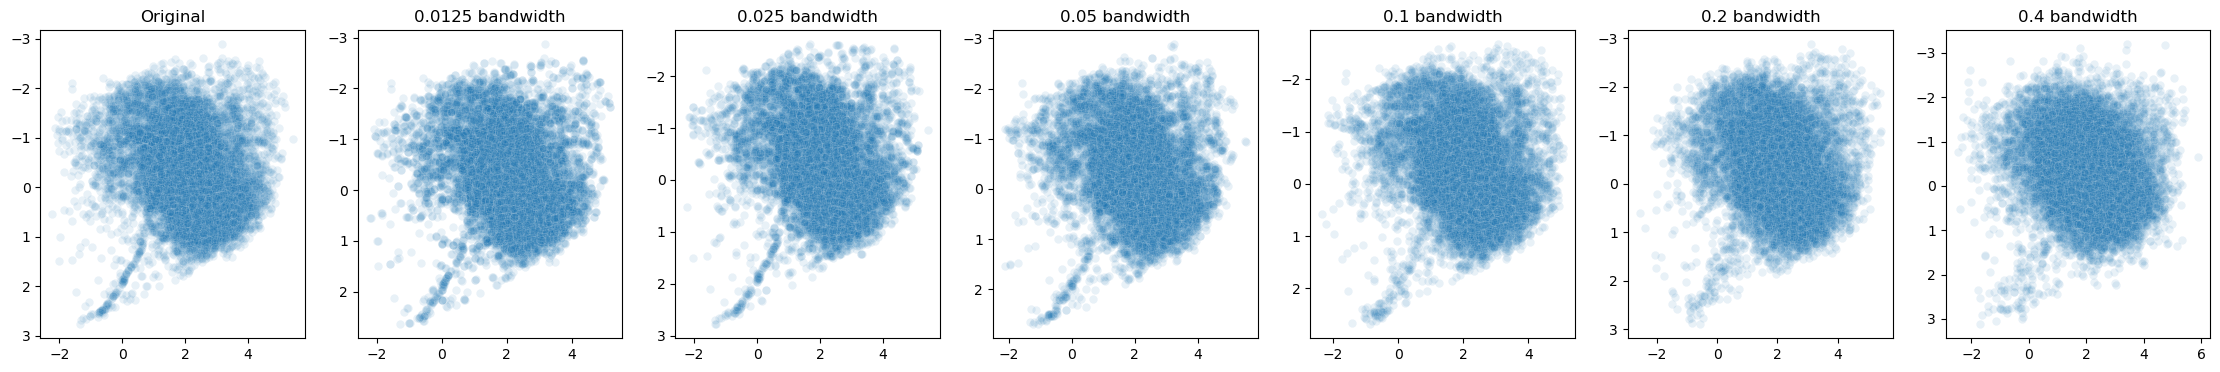
\includegraphics[width=1\linewidth]{images/gaussian-kde-bandwidth.png}
    \caption{Original style distribution compared to resampled distributions.}
    \label{fig:gaussian_kde_bandwith_plot}
\end{figure}

This approach did slightly better than the Conditional Transformer in terms of perplexity while having a bit worse top-1 accuracy (see Table \ref{tab:style_transformer_performance}). This however was not the case for the large variant, as in terms of perplexity and accuracy it even surpassed the performance of the Transformer model. FFD was improved significantly even in the case of the small variant, it beats even the large Conditional Transformer. These results show that inserting more style-related information is useful, we suppose that it makes the results more diverse hence matching the original distribution.

\begin{table}[!htbp]
    \centering
    \begin{tabular}{lrrrrr}
        \toprule
        Model &  Train Perplexity & Test Perplexity & Train Accuracy & Test Accuracy & FFD \\
        \midrule
        StyleS & 3.495 & 3.473 & 62.25\% & 62.58\% & 1.728 \\
        StyleM & 2.581 & 2.560 & 72.63\% & 72.90\% & 1.139 \\
        StyleL & 2.252 & 2.264 & 76.32\% & 76.31\% & 0.824 \\
        \bottomrule
    \end{tabular}
    \caption{Performance of Style Transformer models.}
    \label{tab:style_transformer_performance}
\end{table}

This architecture is not as easily applicable to a real-world product for sequence generation because of the problems associated with the way styling is handled. Nevertheless, given a genre (or any other desired property), a novel sequence could be generated using a style sampled from a Gaussian KDE weighted by the match to that property (e.g. according to the weight of the genre). Another way would be sequence conditioning, where we could take several reference sequences, whose style we want to recreate and use their average style vector acquired by a feature extractor as the condition. The problem is however that our approach predicts based only on a single style vector and not on the entire style distribution; in contrast, the Conditional Transformer uses genre information which spans a larger portion of the style space. Style interpolation would also be tricky, as the distribution is of a complex shape (traditionally, spherical linear interpolation is used on GANs with Gaussian latent space, which is not applicable in our case). This architecture may also be more vulnerable to recreating the training data sequences. We leave these limitations as a subject of future work.
 
\subsection{Human Evaluation} \label{Human Evaluation}

Since the described metrics are not easily interpretable, we decided to use human evaluation. Our approach tried to measure how difficult it is to trick people into believing a generated sequence is real. As there are not any available survey apps that would suit our purposes, a simple web application was created. The user was greeted with an explanation of the project and data processing methods used. Then, they filled in a section about themselves - their age group, gender, and their experience in music. In the main part, 10 random sequences were shown to the user, who had to guess whether each sequence was real or fake. There was an option to play the sequence of chords as an audio file. The sequences shown to the users were randomly sampled from 1,000 real and 1,000 generated sequences (100 for each model). At the end of the survey, users had the option to leave their email address to later receive their results of how successful they were at guessing - to remain rigorous, these results were not sent to them before ending it. The application also tracked the time it took the users to guess the sequences.

The survey ended a week later after the distribution to a few different groups. A total of 46 valid answers were collected, which is quite a small sample, but we will try to make the most of the data anyway. 22 respondents were male, 24 female, no one chose "other / prefer not to say". 5 respondents were in the age group of 10-15 years (upper bounds are exclusive, e.g. 15 years and 2 months are not in this category), 36 respondents were 15-20 years old, 4 were in the group 20-30 and a single user selected 50+. The age distribution is not unexpected as this survey was distributed mostly to high school students. 14 respondents had 0-1 year of music experience (meaning playing an instrument, composition, or work experience), 2 had 1-3 years, 5 respondents 3-5 years, 13 had 5-10 years, 10 had 10-20 years, and 2 more than 20. The survey was on average finished in 3 minutes and 18 seconds, with a standard deviation of 2 minutes and 33 seconds.

The final average accuracy of respondent answers across all sequences (real or generated) was 50.22\%, not any better than random guessing. Surprisingly, there was no significant correlation between the time it took to finish and the accuracy of the respondent, and experience in the field even had a slight negative correlation with the accuracy. The age of the respondents had a similar tendency as the experience. Even though these effects may disappear with a larger number of respondents, it is interesting to see nonetheless. Both genders did about equally well.

Given the small number of responses, we can only get a rough idea of the real performance. Note that while one may think that instead of using numerous real sequences, we could just divert them to the models, this would destabilize the expected percentage of real and generated samples. We use the term perceived realness to describe the portion of answers that were considered real. Since we are dealing with binary data, the standard error was used to approximate the confidence of our findings. A 95\% confidence margin can be obtained by multiplying the standard error by roughly 1.96. Generally, the real sequences were considered slightly more real than fake, however, the generated sequences had about the same value of perceived realness. The recurrent network got the lowest score. The comparison of different Transformer networks is difficult due to the large uncertainty of about 20\% for the 95\% confidence margin. 

\begin{table}[!htbp]
    \centering
    \begin{tabular}{lrrrrr}
        \toprule
        Model & Seen Samples & Perceived Realness & Standard Error \\
        \midrule
        Real (Reference) & 233 & 57.94\% & 3.23\% \\ 
        RecurrentNet & 21 & 38.10\% & 10.60\% \\
        TransformerS & 23 & 69.57\% & 9.59\% \\
        TransformerM & 30 & 53.33\% & 9.11\% \\
        TransformerL & 23 & 60.87\% & 10.18\% \\
        ConditionalS & 17 & 64.71\% & 11.60\% \\
        ConditionalM & 18 & 61.11\% & 11.49\% \\
        ConditionalL & 24 & 54.17\% & 10.17\% \\
        StyleS & 21 & 57.14\% & 10.80\% \\
        StyleM & 23 & 56.52\% & 10.34\% \\
        StyleL & 27 & 62.96\% & 9.29\% \\
        \bottomrule
    \end{tabular}
    \caption{Human evaluation results.}
    \label{tab:human_evaluation}
\end{table}

In conclusion, given our data processing methods and other limitations, it seems that the Transformer models and their variants generated sequences practically indistinguishable from real ones, although further research should be done with a larger number of participants to confirm these findings.

\subsection{Model Performance Overview}

\begin{table}[!htbp]
    \centering
    \begin{tabular}{lrrrrr}
        \toprule
        Model & Parameters & Perplexity & Top-1 Accuracy & FFD & Perceived Realness \\
        \midrule
        RecurrentNet & 376,683 & 4.851 & 56.59\% & 9.290 & 38.10 $\pm$ 20.77\%  \\
        TransformerS & 433,419 & 3.123 & 69.05\% & 3.201 & 69.57 $\pm$ 18.80\% \\
        TransformerM & 1,100,715 & 2.677 & 73.91\% & 2.814 & 53.33 $\pm$ 17.85\% \\
        TransformerL & 2,883,915 & 2.513 & 76.04\% & 2.316 & 60.87 $\pm$ 19.95\% \\
        ConditionalS & 535,115 & 3.521 & 64.81\% & 2.998 & 64.71 $\pm$ 22.72\% \\
        ConditionalM & 1,414,075 & 2.774 & 72.99\% & 2.076 & 61.11 $\pm$ 22.52\% \\
        ConditionalL & 3,780,651 & 2.562 & 75.14\% & 1.848 & 54.17 $\pm$ 19.93\% \\
        StyleS & 541,579 & 3.473 & 62.58\% & 1.728 & 57.14 $\pm$ 21.17\% \\
        StyleM & 1,424,715 & 2.560 & 72.90\% & 1.139 & 56.52 $\pm$ 20.26\% \\
        StyleL & 3,796,491 & 2.264 & 76.31\% & 0.824 & 62.96 $\pm$ 18.22\% \\
        \bottomrule
    \end{tabular}
    \caption{Comparison of the models.}
    \label{tab:model_comparison}
\end{table}

The number of parameters as well as the performance of the models can be seen in Table \ref{tab:model_comparison}. Perplexity and top-1 accuracy are calculated on the test set, the perceived realness confidence intervals denote 95\% confidence.

\FloatBarrier

\subsection{Showcase of Generated Samples}

Below, there are three non-cherrypicked chord sequences generated by each model. They were truncated to 24 chords to fit into a reasonable space. Various other generated sequences can be found on the GitHub repository in a tokenized representation.

\noindent \textbf{Recurrent Net}

\begin{itemize}[noitemsep,topsep=0pt]
    \item D G D A D G D A D G A D G D G D G D G D G D G D...
    \item F\# G\# A\#m F\# C\# G\# A\#m F\# G G\# A\#m F\# G\# Fm A\#m F\# D\#m G\# C\# F\# G\# C\# F\# G\#...
    \item D\#m7 Badd9 G\#m D\#m7 C\#m7 D\#m7 G\#m D\#m7 Emaj7 D\#m7 C\#m7 D\#m7 Emaj9 D\#m7 G\#m7 C\#m7 Amaj9 D\#m7 Badd9 F\#m Emaj7 D\#m7 Badd9 D\#m7...
\end{itemize}

\noindent \textbf{Transformer S}

\begin{itemize}[noitemsep,topsep=0pt]
    \item B C\#m E C\#m A C\#m E B F\#7 B C\#m E C\#m B G\#m C\#m E G\#m C\#m E G\#m
    \item A\#m7 D\#7 G\#maj7 G\# A\#m7 D\#7 G\#maj7 A\#m D\#7 G\#maj7 A\#m D\#7 G\#maj7 A\#m D\#7 G\#maj7 A\#m D\#7 G\#maj7 A\#m D\#7 G\#maj7 A\#m D\#7...
    \item G C D G Em C D G C G Em C D G C G Em C D G Em Bm G D...
\end{itemize}

\noindent \textbf{Transformer M}

\begin{itemize}[noitemsep,topsep=0pt]
    \item D\# F A\# A\#maj7 Cm7 F A\# A\#maj7 Cm7 F A\# Gm7 D\# A\# A\#maj7 Cm7 F A\# F A\# A\#maj7 Cm7 F A\#...
    \item C A\# C A Dm A7 Gm7 C\#aug A7 Dm A\# A7 Dm7 A7 Dm C A\# C Dm A\# C Dm A\# A7...
    \item D\#m C\#7 F\# D\#m C\#7 F\# B F\# D\#m B F\# C\# B C\# F\# D\#m C\#7 F\# B F\# C\# B F\# D\#m...
\end{itemize}

\noindent \textbf{Transformer L}

\begin{itemize}[noitemsep,topsep=0pt]
    \item Bmaj7 D7 Am7 D7 G A\#7 Am7 D7 Gmaj7 Em Am7 D7 Gmaj7 Am7 G7 D7 Am7 D7 Gmaj7 C9 Bmaj7 G\# Am7 D7...
    \item Gm Dm Gm Dm Gm Dm Gm Dm Gm Dm Gm Dm Gm Dm Gm Dm Gm
    \item C\# D\# G\# D\# G\# D\# G\# D\# G\# D\#7 G\# C\# D\# G\# D\# G\# D\# G\# D\#7 G\# C\# D\# G\# D\#...
\end{itemize}

\noindent \textbf{Conditional Transformer S}

\begin{itemize}[noitemsep,topsep=0pt]
    \item B C\#m A B C\#m A B C\#m A B A B A B C\#m A B C\#m A B E A B C\#m...
    \item Dm Am A\# F Dm Am A\# C F Dm Am Gm A\# F Dm Am A\# F Dm Am A\# F Dm Am...
    \item A A7 D7 G A7 D7 G A7 D7 G A7 D7 G A7 D7 G A7 D7 G A7 D7 G A7 D7...
\end{itemize}

\noindent \textbf{Conditional Transformer M}

\begin{itemize}[noitemsep,topsep=0pt]
    \item G A D D7 G Gm6 A D G D Em7 A D A D Bm G A D
    \item C\# F\# B F\# C\# F\# A\#m B F\# C\# F\# G\#m B F\# C\# F\# G\#m B F\# C\# F\# A\#m B F\#...
    \item F\#m G\#m F\#m G\#m C\#m E F\#m G\#m F\#m G\#m C\#m E F\#m G\#m C\#m E F\#m G\#m C\#m E F\#m G\#m C\#m E...
\end{itemize}

\noindent \textbf{Conditional Transformer L}

\begin{itemize}[noitemsep,topsep=0pt]
    \item B E A B E A B E A B E A B E A B E A B E A B E A...
    \item A\#m D\#7 D\# C\# G\# A\#m D\#7 G\# A\#m D\#7 Cm7 D\#7 C\# G\# A\#m D\#7 G\# A\#m D\#7 G\# Fm A\#m D\#7 Cm7...
    \item G\# C\# G\# C\# G\# C\# G\# C\# G\# C\# G\# C\# G\# C\# G\# C\# G\# C\# G\# C\# G\# C\# G\# C\#...
\end{itemize}

\noindent \textbf{Style Transformer S}

\begin{itemize}[noitemsep,topsep=0pt]
    \item G D Bm D\# C G Em C Dm G A F D\# C\#m D Gm C F D\# F D\# A\# A D\#...
    \item G\# A\#m7 G\# D\# G\# D\# A\#m7 G\# D\# G\# C\# A\#m7 D\# G\# C\# D\# G\# D\# C\# A\#m7 D\# G\# D\# C\#...
    \item A\# Dm A\# Gm Cm A\# D\# A\# Gm Cm A\# A7 G\# D\# A\# Gm Cm A\# D\# A\# A7 D\#maj7 D\#m D\#...
\end{itemize}

\noindent \textbf{Style Transformer M}

\begin{itemize}[noitemsep,topsep=0pt]
    \item C\# G\# E F\# D\# F\# G\# C\# G\# E F\# C\# G\# E F\# C\# G\# G\#m E F\# D\#m E F\# C\#...
    \item A\# Gm Dm C C7 F Dm A\# F Dm A\# Gm Dm C Dm A\# Gm Dm C Dm A\# Gm A5 Dm...
    \item B C\# D\#m B C\# D\#m B C\# D\#m B C\# D\#m B C\# D\#m B C\# F\# C\# F\# C\# F\# C\# F\#...
\end{itemize}

\noindent \textbf{Style Transformer L}

\begin{itemize}[noitemsep,topsep=0pt]
    \item D G Bm D G Bm D G Bm D Cmaj7 Bm D G D Em Bm D A D Gmaj7 G D Em...
    \item G\#m7 C\#m6 A9 F\#7 C\#m7 F\#7 C\#m6 Bmaj7 G\#m7 C\#m6 A9 G\#7 C\#m7 F\#7 C\#m6 Bmaj7 G\#m7 C\#m6 A9 G\#7 C\#m7 F\#7 C\#m6 Bmaj7...
    \item Em A Em D Em A Em Bm C\#m F\#m Am D Em Bm C\#m F\#m Am D Em Bm C\#m F\#m C\#m D...
\end{itemize}

\section{Web Application}

\subsection{Introduction}

Deep learning models can be only as useful as the context in which they are used, so to make the result of our work usable for the public, we decided to create a web application centered around our models. The main idea was to help musicians, especially those starting their journey, compose beautiful chord progressions by suggesting the next chord in the context of the previous chords. A user would see their sequence and get suggestions on what to do next, enabling an effective exploration of the landscape of possibilities.

Similar products already exist, but they are usually paid for, unpractical to use, or limited in other ways. The creation of an open-source, free-to-use AI-powered tool could therefore allow anyone to compose chord progressions simply. The app could also serve as a way to learn a part of music theory, as chord progressions and their notation are quite complex to understand.

\subsection{Web Stack}

Next.js 14 \cite{nextjs14.0.4} was chosen as the web development framework. TypeScript was used instead of JavaScript and Tailwind CSS \cite{tailwindcss3.3.6} was used as the library for styling. Zustand \cite{zustand4.4.7} served as the state management library, ONNX runtime \cite{onnxruntime1.16.3} was employed to run the AI models, Tone.js \cite{tonejs14.7.77} did the job of an audio playback library for the composed chord progressions.

\subsection{Architecture}

\begin{figure}[!htbp]
    \centering
    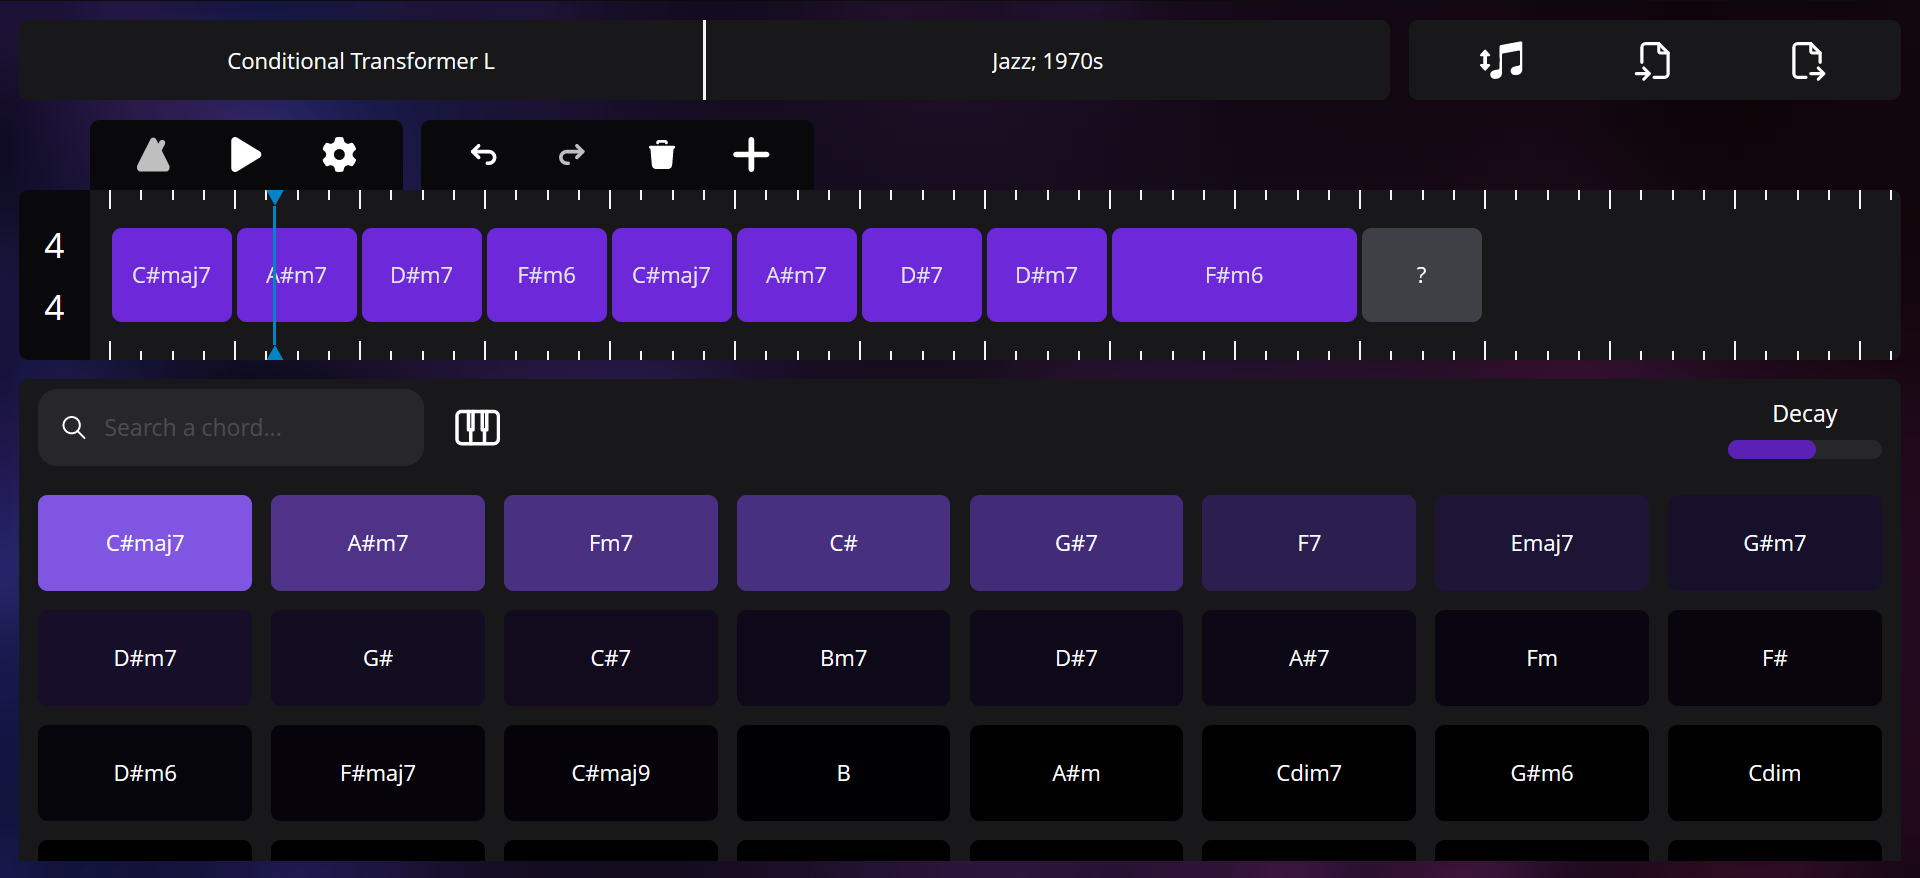
\includegraphics[width=1\linewidth]{images/app-screenshot.png}
    \caption{The web application.}
    \label{fig:app_screenshot}
\end{figure}

\textbf{General structure.} The UI is comprised of a few components, including the timeline, suggestions, model/style selection, transpose/import/export menu, and a chord variation pop-up menu. Keyboard shortcuts, also sometimes called hotkeys, are available for most of the functions of the app. When you hover over an element of a component, it shows you what happens on click as well as the shortcut for it. The state of the app, including the chord progression, selected model and style, signature, tempo, and default variants, are automatically saved locally in the browser, so the user will not lose progress unless they delete the site data. We will delve into each of the components in depth, going in a natural order as a user might explore the app.

\textbf{Timeline.} At the heart of the app is the timeline, a component in which the chord progression is built. The controls are similar to that of video editors, scrolling can be used to zoom in/out, and dragging the middle mouse moves the view.

A new chord can be added by clicking the plus icon above the timeline, or by the hotkey \texttt{A}. All newly added chords are blank by default (denoted by a question mark), they can be changed for a different chord in the suggestions. By clicking on any chord in the timeline, you select it, which is signalized by appearing in a lighter color. Clicking on an already selected chord deselects it, alternatively, you can use the hotkey \texttt{Esc}. Arrow keys can be used to navigate the selection of chords. Every time a chord is selected (either by clicking it or by arrow keys), it is played to make it easier to comprehend what the user is composing. Adding a new chord either appends it to the end of the sequence or if any chord is selected, the new chord is inserted right after it. There can be a maximum of 255 chords after processing them (merging consecutive and ignoring blank chords).

The selected chord can be deleted by clicking the thrash bin icon (hotkey \texttt{Del}). The duration a chord spans can be changed by resizing it from the right edge (hover over the right edge of a chord, click, then drag it); the value snaps to the beats. All changes that are made to the sequence, including the selection and deselection of chords, are recorded (up to 64 steps), you can undo/redo them by the icons to the left of the thrash bin or by hotkeys \texttt{Ctrl + Z}/\texttt{Ctrl + Y}.

Left to the add/delete/undo/redo controls are the playback controls. The middle icon starts and pauses playback (\texttt{Space}). When the sequence a playing, the current timestep is visualized by the blue moving playhead. The position of the playhead can be changed by clicking or dragging on the time ticks (the top and bottom part of the timeline around the chords) both while playing and not. Once the playhead reaches the end of the sequence, the playback ends and the playhead jumps back to the start of the sequence. The left metronome icon enables and disables the metronome (\texttt{M}). The tempo of the playback in beats per minute can be changed from the right settings icon.

The signature (the number of beats per measure) of the chord progression can be customized by clicking on the signature in the left part of the timeline. When the signature changes, the chord durations remain constant, adapting to the new values. The signature is also visualized by the ticks at the top and bottom of the timeline, where a slightly larger tick denotes the boundary of two measures.

\textbf{Suggestions.} When any chord is selected, the suggestions for the chord given its preceding chords are available. You can scroll to see more suggestions. By clicking on any suggested chord, the selected chord is replaced with the suggestion, and the new chord is played. The suggested chords are colored from purple to black and sorted by the probability predicted by the model. The coloring decay can be controlled by the decay slider at the top right corner. Note that logarithmic coloring is used instead of linear to make less probable chords still visible, which provides a more natural way to think about the predictions of the model.

Specific chords can also be searched from the top left search bar, if you do not find what you want, try enabling \textit{Include variants}, as the chord you are searching for may be a variant of another base chord (e.g. Am7 and C6 are variants of the same chord, as they are the inversions of each other). You can also filter the chords by the notes used under the piano icon, which opens a virtual keyboard on which you can enter the notes by clicking on individual keys. When any search query is applied, an icon to clear the search results is shown (queries are cleared when clicked on).

Suggestions may take a while to load, as the model runs locally in the browser using the ONNX runtime. Note that once a suggestion is made, it is cached for later use (up to 32 predictions are cached, after that the first ones are removed to free the memory).

\textbf{Model and style selection.} From the upper left menu, the users can select the model they want to use for suggestions by clicking on it and selecting another variant from the dropdown. A larger model may produce better suggestions at the cost of a longer inference time. When a Conditional model is selected, a style (respectively the condition) menu can be opened by clicking the right part of this component. Two tabs are included in the style selection, the genre and the decade. By clicking on any style element from the dropdown, its state changes (enabling/disabling it). Multiple genres and decades can be selected. Additionally, the relative weighting of each of the styles can be specified. We suggest using small integer values to make it easy to think about; behind the scenes, the weights get normalized to sum to one either way. Since the applied style changes the predictions of the models, the suggestions are updated on every change. The genres are sorted by their occurrence in the dataset. Style Transformer models were not added due to the difficulties associated with them (see the last paragraph of section \ref{Style Transformer}). 

\textbf{Transpose/Import/Export.} The chord sequence can be easily transposed under the left icon of this menu. Positive integer values transpose by that number of semitones up, while negative transpose down. The sequence can be exported to a .chseq or .mid format under the right icon, corresponding to a custom format (preferred for saving/loading sequences; it is just JSON in the background), and MIDI (for use in other music production software), respectively. Imports are done under the middle icon, again, you can import a .chseq or .mid file. Manually editing the .chseq file may cause a corrupted state of the app after import, which can be fixed by clearing the site data. Imported MIDI files should be single track, only with the chords in a condensed format (without arpeggios, strummed chords, and other variants), without other voices (such as percussion and melodies). If a chord is not recognized or there are no notes in the MIDI file (corresponding to a rest), it will be replaced by the unknown token (denoted by a question mark).

\textbf{Chord variants.} Given the data processing methods used, the inversions of chords as well as other voicings are mapped to the same token. Therefore, to make the app more intuitive, the user can choose the variant of any chord, both in the timeline and in the suggestions. This menu can be opened by right-clicking on any chord. A visualization of the notes the chord is comprised of is shown on a virtual keyboard and other chord variants are under it. Upon clicking on any other variant, it will be again visualized and played. When this menu is open from the timeline, the newly selected variant can be either applied once (only to that chord) or to all (replacing all of the same chords with this variant). When it is open from the suggestions, it can be used once (replacing the selected chord with this variant) or set as default (which makes it the preferred variant in the suggestions). You can close this menu from the close icon (alternatively \texttt{Esc}).

Even though it may be tempting to use chord variants to compose the chord voicings, this is not a recommended approach, as variants were only added to make searching for chords more intuitive and allow multiple possible notations to be used. Instead, this app should only be utilized for the base chord progressions and the voicings should be made in another music production software (after exporting it to the MIDI format).

\subsection{Other Aspects}

\textbf{Models.} Since the models are not that computationally expensive, they were deployed on the edge. The models were converted to the ONNX format and are run locally in the browser using ONNX Runtime Web. To make the data the model receives processed in the same way as what it was trained on, consecutive and unknown chords are ignored. The duration and the variant of the chord do not influence the predictions. Ensuring that ONNX works in the browser was problematic due to the need for a web assembly package at a specific static path, which requires different build and development copy webpack plugin path settings with Next.js 13+.

\textbf{Progressive Web App.} This application can also be installed on desktop devices as a PWA.

\textbf{Icons.} The icons in the app come from Font Awesome Icons V6 \cite{fontawesome6} and Tabler Icons \cite{tablericons}. The transposition icon is made from two icons. The app logo was created using Inkscape \cite{inkscape1.2.2} and should represent a hybrid of a soundwave and a digital brain.

\textbf{Sounds.} The piano sound used for playback as well as the ticking sound of the metronome are from the Tone.js audio library \cite{TonejsAudio}.

\textbf{Deployment.} This app was not deployed online as a part of this graduate project, however, a privately hosted version may be available in the future.

\textbf{Support.} This app is currently only supported on desktop devices. It was built in a Chromium-based browser, so this app may be unstable in other browsers.

\section{Future Work}

Even though this project produced a useful tool, a lot could be improved. In this section, we will describe some approaches to try in the future.

One of the biggest limitations of this work is that it does not consider chord durations. Now that there is a decent map to get the symbol of chords just based on the notes, a different dataset could be used. Given a large dataset of MIDI files, their chord progressions could be extracted and processed in a way to obtain the chords and their durations. A model could then be trained to accept the durations of the chord in a similar way as positional encoding, prediction of the duration of a chord could be done by extending the possible prediction tokens, one for each duration (a single duration output would not be enough as different chords of different durations fit in each context). In a final product, the user could then explore the chords with the duration, or the probabilities of a chord by merging all of the possible durations (constructed by summing them), which would work similarly to our app, just that the durations of chords would be considered during inference.

Another aspect that is not accounted for is the different variants of chords. A more powerful tool trained on a larger dataset could predict the probabilities for each of them independently. A user of such an app could then collapse them to include them under the same token (same as our app, just that under variations the probabilities would be visible) or see them separately. This tool could theoretically produce chord voicings in a meaningful way, contrary to our work that focuses only on the pitch classes used.

If a large enough dataset with descriptions of the songs was obtained, our conditional model could then be used together with a (possibly pre-trained) language Transformer to enable the generation of sequences based on text descriptions.

The application of a style is still problematic, and a generative adversarial learning method for discrete sequences with Transformers could be developed. Such a breakthrough would revolutionize the field of symbolic music generation, as such problems could be then treated similarly to image generation.

\section{Conclusion}

In this project, we have presented ChordSeqAI, a tool utilizing deep learning for generating chord sequences. We undertook a comprehensive approach, starting from data acquisition and analysis, through the development and training of various models, to the final use in a web application.

The exploration and analysis of a large dataset of chord sequences have revealed interesting patterns in chord progressions across different genres and decades. Our deep learning models range from a basic recurrent network to more complex Transformer architectures. The introduction of conditional and style-based Transformers has further enriched our tool's capabilities, allowing for a more controllable generation of chord sequences that are indistinguishable from real samples. The development of a web application has been a crucial step in making our tool accessible to a broader audience. By integrating our models into an intuitive interface, we have opened up the possibility for both amateur and professional musicians to explore and experiment with chord progressions.

In conclusion, ChordSeqAI represents an attempt to make the fusion of artificial intelligence and music composition available to anyone. By simplifying and enriching chord progression composition, where the artist is in charge of the generative process, ChordSeqAI aims to be a supportive tool rather than a replacement, enhancing creativity and offering new perspectives in musical composition. It is a step towards democratizing music creation, where deep learning combined with artistry paves the way for uncharted territories in creativity.

\section{Additional Resources} \label{Resources}

The code used for this project is available on GitHub under the MIT license, the human evaluation web application is not included, as it was made as a quick and unpolished alternative to other survey services.

\begin{itemize}
    \item Data, models, evaluation: \href{https://github.com/StudentTraineeCenter/chord-seq-ai}{https://github.com/StudentTraineeCenter/chord-seq-ai}

    \item Web Application: \href{https://github.com/StudentTraineeCenter/chord-seq-ai-app}{https://github.com/StudentTraineeCenter/chord-seq-ai-app}
\end{itemize}

\printbibliography

\end{document}
